
\documentclass{mproj}
\usepackage{graphicx}

\usepackage{url}
\usepackage{fancyvrb}
\usepackage[final]{pdfpages}
\usepackage{times}

%\usepackage[nottoc,numbib]{tocbibind}
\usepackage[nottoc]{tocbibind}

% for alternative page numbering use the following package
% and see documentation for commands
%\usepackage{fancyheadings}


% other potentially useful packages
%\uspackage{amssymb,amsmath}
%\usepackage{url}
%\usepackage{fancyvrb}
%\usepackage[final]{pdfpages}
\usepackage{CTEX}
\usepackage{comment}

\usepackage[section]{placeins} % 添加这个以限制浮动体跨越节的边界

\usepackage{listings}
\usepackage{xcolor}  % 用于定义颜色

\usepackage{amsmath}

\usepackage{hyperref}
\usepackage{cleveref}
\crefname{figure}{Figure}{Figures} % 设置 \cref 引用图像的格式

\begin{document}

%%%%%%%%%%%%%%%%%%%%%%%%%%%%%%%%%%%%%%%%%%%%%%%%%%%%%%%%%%%%%%%%%%%
%Towards Faster Parallelism: Performance-Driven Workstealing Scheduling in YewPar
\title{Towards Faster Combinatorial Search: Performance-Driven Workstealing Policy in YewPar}
\author{Hao Xie}
\date{31th August 2023}
\maketitle
%%%%%%%%%%%%%%%%%%%%%%%%%%%%%%%%%%%%%%%%%%%%%%%%%%%%%%%%%%%%%%%%%%%

%%%%%%%%%%%%%%%%%%%%%%%%%%%%%%%%%%%%%%%%%%%%%%%%%%%%%%%%%%%%%%%%%%%
\begin{abstract}

    % \begin{comment}
    % 精确组合搜索对于包括约束编程、图匹配和计算代数在内的广泛应用都是必不可少的。
    % 而并行化计算也是加速组合搜索的重要手段之一,
    % Workstealing是实现并行化计算的一种重要策略,
    % 当有节点的计算资源空闲时,通过窃取其它节点的剩余任务来利用空闲的计算资源,从而提高整体性能。
    % YewPar is a very good parallel framework designed for combinatorial search.
    % It provides a set of powerful skeletons and policies that allow developers to easily parallelize their search algorithms.
    % 但是它的workstealing策略是偏向随机挑选有任务的节点进行任务窃取,
    % 这往往会导致不必要的开销和延迟,
    % 我们的目标是通过设计一种新的workstealing策略来提高基于YewPar框架的应用的运行速度.

    % 为此我们设计并实现了一种新的基于各节点程序的多项性能参数来实时调整任务窃取的目标节点的Performance-Driven Workstealing Policy框架,
    % 它的主要理念是通过多种方式例如去窃取负载较高的节点的任务来达到接近负载均衡的状态等,
    % 从而缩短最后完成任务的worker的时间,
    % 并且通过减少不必要的探测时间来缩短无任务worker的饥饿时间,
    % 最终缩短基于YewPar的应用在并行情况下的运行完成时间.

    % 并且我们对改进workstealing策略后的YewPar进行了评估,
    % 评估在具有多核机器的Beowulf集群上进行,
    % 结果表明,改进后的YewPar在不同节点数量和负载情况下相比原YewPar能够获得更好的性能,
    % 能在不影响搜索结果的情况下不同程度的有效缩短基于YewPar的搜索应用的执行时间,
    % 在多数情况下对于其运行速度的提升非常显著.
    % \end{comment}

    Exact combinatorial search is indispensable for a wide range of applications, including constraint programming, graph matching, and computational algebra.
    Parallel computation serves as a vital method to accelerate these combinatorial searches.
    Workstealing is a key strategy for achieving parallelization.
    By pilfering remaining tasks from other nodes when a node's computational resources are idle,
    it capitalizes on the available computational resources, thereby enhancing the overall performance.
    YewPar is an exemplary parallel framework designed specifically for combinatorial search.
    It offers a suite of potent skeletons and policies, enabling developers to seamlessly parallelize their search algorithms.
    However, its Workstealing strategy predominantly leans towards randomly selecting nodes with tasks for pilfering.
    This often results in unnecessary overheads and delays.
    Our objective is to boost the execution speed of applications based on the YewPar framework by introducing a novel Workstealing strategy.

    To this end, we have devised and implemented a new Performance-Driven Workstealing Policy framework that dynamically adjusts the target node for task pilfering based on multiple performance parameters of each node's program.
    The core philosophy behind this approach is to strive for near load-balancing by predominantly pilfering tasks from nodes with higher loads, thereby minimizing the completion time of the last finishing worker.
    Moreover, by curtailing unnecessary probing time, it significantly reduces the starvation time of task-less workers.
    Ultimately, this results in a marked reduction in the execution time of YewPar-based applications in parallel scenarios.
    At the same time, since the collected performance parameters are currently available in the most advantageous Workstealing frameworks and can be obtained simply,
    Therefore, it has good portability and versatility, and it can be more easily transplanted to other platforms and frameworks.

    We have also evaluated the improved YewPar with the enhanced Workstealing strategy.
    The evaluation was conducted on a Beowulf cluster equipped with multi-core machines.
    The outcomes indicate that, compared to the original YewPar, the revamped YewPar yields superior performance under various node quantities and loads.
    It can significantly trim the execution time of search applications based on YewPar without compromising the search results.
    In most instances, the enhancement in its execution speed is remarkably pronounced.

    \textbf{Keywords:} Combinatorial Search, Parallel Computation, Workstealing, YewPar, Performance-Driven Policy, Beowulf Cluster.

\end{abstract}
%%%%%%%%%%%%%%%%%%%%%%%%%%%%%%%%%%%%%%%%%%%%%%%%%%%%%%%%%%%%%%%%%%%

%%%%%%%%%%%%%%%%%%%%%%%%%%%%%%%%%%%%%%%%%%%%%%%%%%%%%%%%%%%%%%%%%%%
\educationalconsent


%%%%%%%%%%%%%%%%%%%%%%%%%%%%%%%%%%%%%%%%%%%%%%%%%%%%%%%%%%%%%%%%%%%

\newpage
%%%%%%%%%%%%%%%%%%%%%%%%%%%%%%%%%%%%%%%%%%%%%%%%%%%%%%%%%%%%%%%%%%%
\section*{Acknowledgements}

It took months almost entirely to focus on this project and do this dissertation.
As a student unfamiliar with the topic initially,
I have done much work with effort and interest to gain knowledge regarding the YewPar framework,
Combinatorial Search and Workstealing concepts related to the project.

So, I would like to thank my supervisor Blair Archibald, who helped me a lot in completing this project.
He discussed the project with me every week and gave me a lot of advice, which benefited me
greatly.

I would also like to thank my family for their love and support throughout my life. Also, my
roommates and other friends, who encouraged me a lot during my project.

%%%%%%%%%%%%%%%%%%%%%%%%%%%%%%%%%%%%%%%%%%%%%%%%%%%%%%%%%%%%%%%%%%%
\tableofcontents
%%%%%%%%%%%%%%%%%%%%%%%%%%%%%%%%%%%%%%%%%%%%%%%%%%%%%%%%%%%%%%%%%%%

%%%%%%%%%%%%%%%%%%%%%%%%%%%%%%%%%%%%%%%%%%%%%%%%%%%%%%%%%%%%%%%%%%%
\chapter{Introduction}\label{intro}

精确组合搜索对于包括约束编程、图匹配和计算代数在内的广泛应用都是必不可少的。
而组合问题是通过系统地探索搜索空间来解决的,这样做在理论上和实践中都很难计算,
其中精确搜索则是探索整个搜索空间并给出可证明的最佳答案。
概念上精确的组合搜索通过生成和遍历代表备选选项的(巨大的)树来进行。
结合并行性、按需树生成、搜索启发式和剪枝可以减少精确搜索的执行时间。
由于巨大且高度不规则的搜索树,并行化精确组合搜索是极具挑战性的.

而其中有名为YewPar\cite{10.1145/3332466.3374537}的框架,这是第一个用于精确组合搜索的可扩展并行框架。
YewPar旨在允许非专业用户从并行中受益;
重用编码为算法骨架的并行搜索模式(reuse parallel search patterns encoded as algorithmic skeletons);
并能在多个并行架构上运行。

与此同时,随着并行计算和多核处理器的普及,有效的任务调度变得越来越重要.
能并行加速搜索是YewPar的一个关键特性,这是通过各个节点的多个worker在本地任务池无任务时向其它节点的任务池窃取任务来实现节点空闲资源的利用。
而YewPar在本地任务池无任务时,是随机选取节点来窃取任务的,
其中Workstealing是一种被广泛研究和应用的并行调度策略,
它允许空闲的处理器从繁忙的处理器中“窃取”任务。
然而,很多如YewPar这样的内部Workstealing调度器往往采用偏随机窃取的策略,
这往往会导致不必要的开销和延迟,浪费了大量试探窃取任务的时间,同时导致各节点的相对负载不均衡,延长了最终完成的时间。
目前也有很多关于workstealing的改进,但是不能很好的兼顾到轻量化,去中心化,高性能,通用化等特性.

我们的目标是通过改进YewPar的Workstealing策略来提高其性能,
为此本文提出了新的Performance-Driven Workstealing Policy框架,
它的主要理念是通过尽量去窃取负载较高的节点的任务来达到接近负载均衡的状态,从而缩短最后完成任务的worker的时间,
并且通过减少不必要的任务探测和窃取时间来缩短无任务worker的饥饿时间,
最终缩短基于YewPar的应用在并行情况下的运行完成时间.

它具有多项功能,
能定期监测与传输多项有价值的数据,
并计算缓存最优窃取目标节点,
它能够通过自研的架构和数据处理算法以低成本搜集和分享多项性能指标,
如各节点的负载情况、各节点剩余任务数量和各节点的通讯延迟,
并通过自研的Time-Optimized Workstealing Strategy算法计算出最优窃取目标节点并缓存和定时刷新,
当有worker空闲时便能直接从缓存获取最近一段时间的最优窃取目标,
从而能很好的在多节点去中心化的设计下以较低成本缩短完成全部任务所需的时间.
同时由于其收集的性能参数是当前有利用到Workstealing的框架都具有并可以采用较为简单的方式获取,
所以它具有很好的轻量化,可移植性和通用性特点,可以更轻松地将这套方案移植到其它平台与框架上并不必担心对系统造成的额外负担.

本文对具体的设计与实现细节进行了剖析,
其中Performance-Driven Workstealing Policy在搜集性能参数时采用了平台无关与去中心化的设计,
一方面并不涉及具体的系统参数调用命令,而是从YewPar内部和底层的HPX\cite{10.1145/2676870.2676883}框架进行数据收集,从而能够在不同的硬件平台上正常运行;
另一方面没有单一的节点负责收集所有节点的性能参数,而是各节点各自收集本地的性能参数,并通过HPX的分布式通信机制分享本地处理后的数据,
同时获取其它节点数据进行本地最优窃取目标计算,从而避免了单一节点的性能瓶颈.
其中Time-Optimized Workstealing Strategy的核心思想是计算各节点执行本地任务的所需时间的预期和获取节点任务池任务的耗时的预期,
并优先选取所需时间预期最大的节点同时尽量缩短不必要的获取任务的额外耗时,从而降低各节点的worker空闲率的同时缩短完成全部任务所需的时间.
其中定时刷新最优窃取目标缓存的任务由一种动态调整刷新时间的自动刷新任务来主要负责,各节点都会部署一个这样的刷新器,
它通过间隔一个动态时间后执行刷新性能参数信息并计算最优窃取目标最后将最优目标进行缓存来实现刷新最优窃取目标缓存的目的.
而空闲的worker则会在试图获取缓存目标任务失败时进行一次称为辅助刷新的操作,帮助此时可能处在休眠的刷新器进行刷新最优窃取目标缓存的任务.
这些工作结合起来便能够实现Performance-Driven Workstealing Policy的加速效果.

本文还对改进workstealing策略后的YewPar进行了评估,
评估在具有多核机器的Beowulf集群上进行,
结果表明,改进后的YewPar在不同节点数量和负载情况下相比原YewPar能够获得更好的性能,
能在不影响搜索结果的情况下不同程度的有效缩短基于YewPar的搜索应用的执行时间,
在多数情况下对于其运行速度的提升非常显著.


%%%%%%%%%%%%%%%%%%%%%%%%%%%%%%%%%%%%%%%%%%%%%%%%%%%%%%%%%%%%%%%%%%%
\chapter{Survey}\label{survey}


\section{Modern Strategies in Distributed Concurrency}
\subsection{Workstealing}
Workstealing 是并行编程中的一个核心概念。
其主要优点在于分散调度,让每个处理器自主地管理其任务队列,从而显著降低了全局同步所带来的开销.
工作窃取的想法可以追溯到20世纪80年代Multilisp编程语言的实现和并行函数式编程语言的工作\cite{10.1145/324133.324234}。
它用于Cilk编程语言的调度程序\cite{BLUMOFE199655}、
Java fork/join框架\cite{lea2000forkjoin}、
.NET任务并行库\cite{leijen2009design}、
和Rust Tokio 运行时\cite{tokio,krill2021tokio}。
和其它众多的并行框架和库。

\begin{figure}[h]
    \centering % 让图片居中显示
    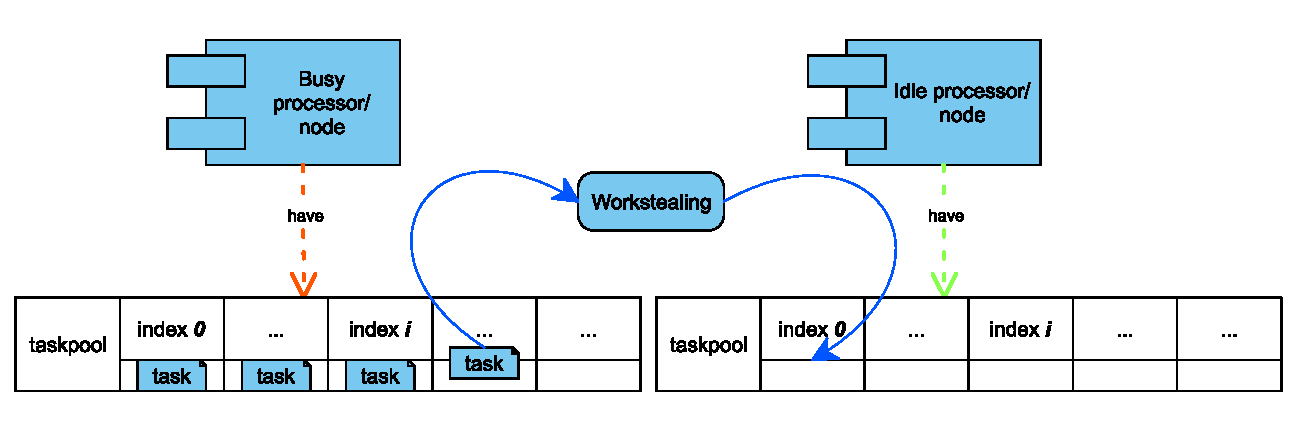
\includegraphics[width=0.98\textwidth]{images/workstealing.pdf} % 插入图片,设置图片宽度为文本宽度的80%
    \caption{Workstealing example} % 提供图片的注解
    \label{fig:workstealing} % 为图片提供一个标签,以便在文档的其他地方引用
\end{figure}
\FloatBarrier

如\cref{fig:workstealing},
在workstealing策略中,系统内的每个处理器都有自己的待执行任务队列.
每个任务都由一系列指令组成,这些指令需要按顺序执行。
在执行的过程中,一个任务还可能生成新的子任务.
这些子任务被初步放入生成它们的任务所在的处理器队列.
当某处理器的任务队列为空时,它会尝试从其他处理器的队列中“窃取”任务.
这样,workstealing 实际上将任务调度到了空闲的处理器上,
并保证了只有在所有处理器都繁忙时才会发生调度开销.\cite{10.1145/1248377.1248396}

与workstealing形成对比的是工作共享策略,
它是动态多线程调度的另一种方法。
在工作共享中,新产生的任务会被立即调度到一个处理器上执行。
相较于此,workstealing减少了处理器间的任务迁移,
因为当所有处理器都繁忙时,这种迁移是不会发生的.\cite{10.1145/324133.324234}

而其中的算法如Blumofe和Leiserson提出的随机化工作窃取算法,
维护了多个执行线程(异步任务)并在P个处理器上进行调度\cite{10.1145/324133.324234}。
每个处理器都有一个双端队列(deque)用于存放线程,
它将deque的两端称为"顶部"和"底部"。
当处理器有当前线程需要执行时,
它会逐条执行线程中的指令,
直到遇到引起四种"特殊"行为中的一种:
\begin{itemize}
    \item “生成”指令会创建一个新的线程。当前线程被放置在deque的底部,处理器开始执行新线程。
    \item “暂停”指令会暂时停止其线程的执行。处理器从其deque的底部弹出一个线程并开始执行。如果deque为空,它开始执行工作窃取。
    \item 某些指令可能导致线程终止。在这种情况下的行为与线程暂停的行为相同。
    \item 指令可能激活另一个线程。这个其他线程被推到deque的底部,但处理器继续执行其当前线程。
\end{itemize}
最初,计算只包含一个线程,并分配给某个处理器,而其他处理器开始为空闲。
任何变为空闲的处理器都开始实际的工作窃取过程,包括以下步骤:
\begin{itemize}
    \item 它随机选择另一个处理器。
    \item 如果另一个处理器的deque非空,它会从deque的顶部弹出最上面的线程并开始执行;
    \item 否则,重复上述过程。
\end{itemize}

但是类似这种随机窃取策略在多节点复杂环境中往往有较大的开销.
这些开销主要来源于“窃贼”在集群中随机地探测节点以寻找“受害者”.
加之集群规模的不均匀分布,这种问题变得更为严重,
导致系统消息量过大以及“窃贼”由于多次窃取失败和网络延迟而产生的长时间饥饿状态.
尽管关于workstealing的优化尝试从未停歇,
例如通过建立固定的"媒人"节点,
让有多余任务的节点和无任务的节点通知媒人节点自己当前的状态,
从而能让"媒人"节点匹配任务饥饿和任务丰富的节点,
从而让无任务节点找到有多余任务的节点进行任务的窃取\cite{10.1145/2851141.2851175},
但是其"媒人"节点的维护和在出现任务饥饿时向"媒人"节点发送查询请求的等待时间等仍然是不可忽视的开销,
同时它只是匹配了有额外任务的节点和无任务的节点使其能进行任务窃取,
但是没有针对节点的各项性能参数情况来进行优化,
可以会导致频繁的发生窃取浪费了不必要的时间;
或者专门针对Multicore Event-Driven Systems设计的窃取策略\cite{5541655},
它特别考虑了事件驱动编程的特点,有效提高在这种环境下的并行度,减少了窃取开销,
但是其但维护任务随机化和延迟窃取策略带来了不少额外的开销,
并且对于非事件驱动的应用不能很好地适用.

还未有一种很好的通用化的低开销、轻量化、跨平台且高效的策略出现。
Workstealing仍主要处于针对各种应用环境进行针对性优化的阶段。
而文本的设计的任务窃取方案是基于各节点性能数据主要是采用基于worker负载情况,各节点剩余任务量和各节点通讯延迟的性能数据,
这些数据可以很轻松的在其它采用Workingstealing策略的框架中获取,
所以具有很好的可移植性和通用性,
可以更轻松地将这套方案移植到除了YewPar以外其它平台与框架上,
而且设计也具有轻量化的特点.

\subsection{The Pitfalls of Locking Mechanisms and the Promise of Lock-Free Designs}\label{survey_lock}
在多线程的优化是一个很热门的领域,
其中锁机制被设计用来解决并发操作中的数据不一致问题,
而Edward A. Lee曾提出锁机制是多线程最主要的问题之一\cite{1631937},
锁会导致线程等待,从而造成性能损耗。在高并发环境下,这种等待可能会导致严重的性能瓶颈。
也会导致当多个线程尝试获取同一个锁时进入竞争状态。
这种竞争状态不仅降低了性能,还可能导致线程饥饿,其中一些线程可能永远无法获取到锁。
Lee强调,尽管有许多方法可以缓解这些问题,
但根本解决方案是寻找替代多线程的编程方法和模型,其中无锁编程就是一个有前景的方向。

而无锁设计目前已有很多优秀的实践,
比如有无锁的并发队列算法,
使得多个线程可以在没有锁的情况下并发地访问和修改队列\cite{10.1145/248052.248106};
还有一种动态的、基于无锁设计的哈希表,由于避免了锁的开销,该设计在高并发环境下可以提供出色的性能\cite{10.1145/564870.564881}.

而本文也借鉴了一些无锁化的设计,
设计了无锁化的数据结构和算法,
让本文的Performance-Driven Workstealing Policy框架在保证数据正确的同时,
避免了锁对性能的影响,
也一定程度保障了本文的框架的轻量化和高性能.


\section{组合搜索}
\begin{comment}
在计算机科学和人工智能中,组合搜索是一种用于在给定的搜索空间中找到解决方案的方法。
经典的组合搜索问题包括解决八皇后难题或评估具有大型游戏树的游戏中的动作,例如黑白棋或国际象棋。
这种搜索特别适用于那些解空间巨大并且不可能穷举所有解决方案的问题。
一些算法保证找到最优解,而另一些算法可能只返回在已探索的状态空间部分中找到的最佳解。
通过分支与限界技术或采用启发式方法,组合搜索能够有效地减少搜索空间,并更快地找到解决方案。
\end{comment}

\subsection{并行组合搜索(Parallel Combinatorial Search)与YewPar}
随着现代计算机硬件的发展,特别是多核处理器和分布式系统的普及,
利用并行性来加速组合搜索已经成为研究的热点.
并行组合搜索的目标是将搜索空间分解成多个部分,以便可以在多个处理单元上同时执行,从而加速解决方案的发现。


并行树搜索可以分类\cite{gendron1994parallel}如下:
(1)并行节点处理(Parallel Node Processing)并行化分支/边界,
例如在GPU上计算Flowshop问题的边界\cite{gmys2016work}。
(2)空间分割,其中并行工作人员推测性地探索搜索树的子树.
虽然子树是独立探索的,但诸如改进边界之类的知识通常在工作人员之间共享以提高性能.
(3)组合方法并行运行竞争搜索,通常使用不同的启发式或边界方法.结合这些方法的混合方法也被使用.

\begin{figure}[h]
    \centering % 让图片居中显示
    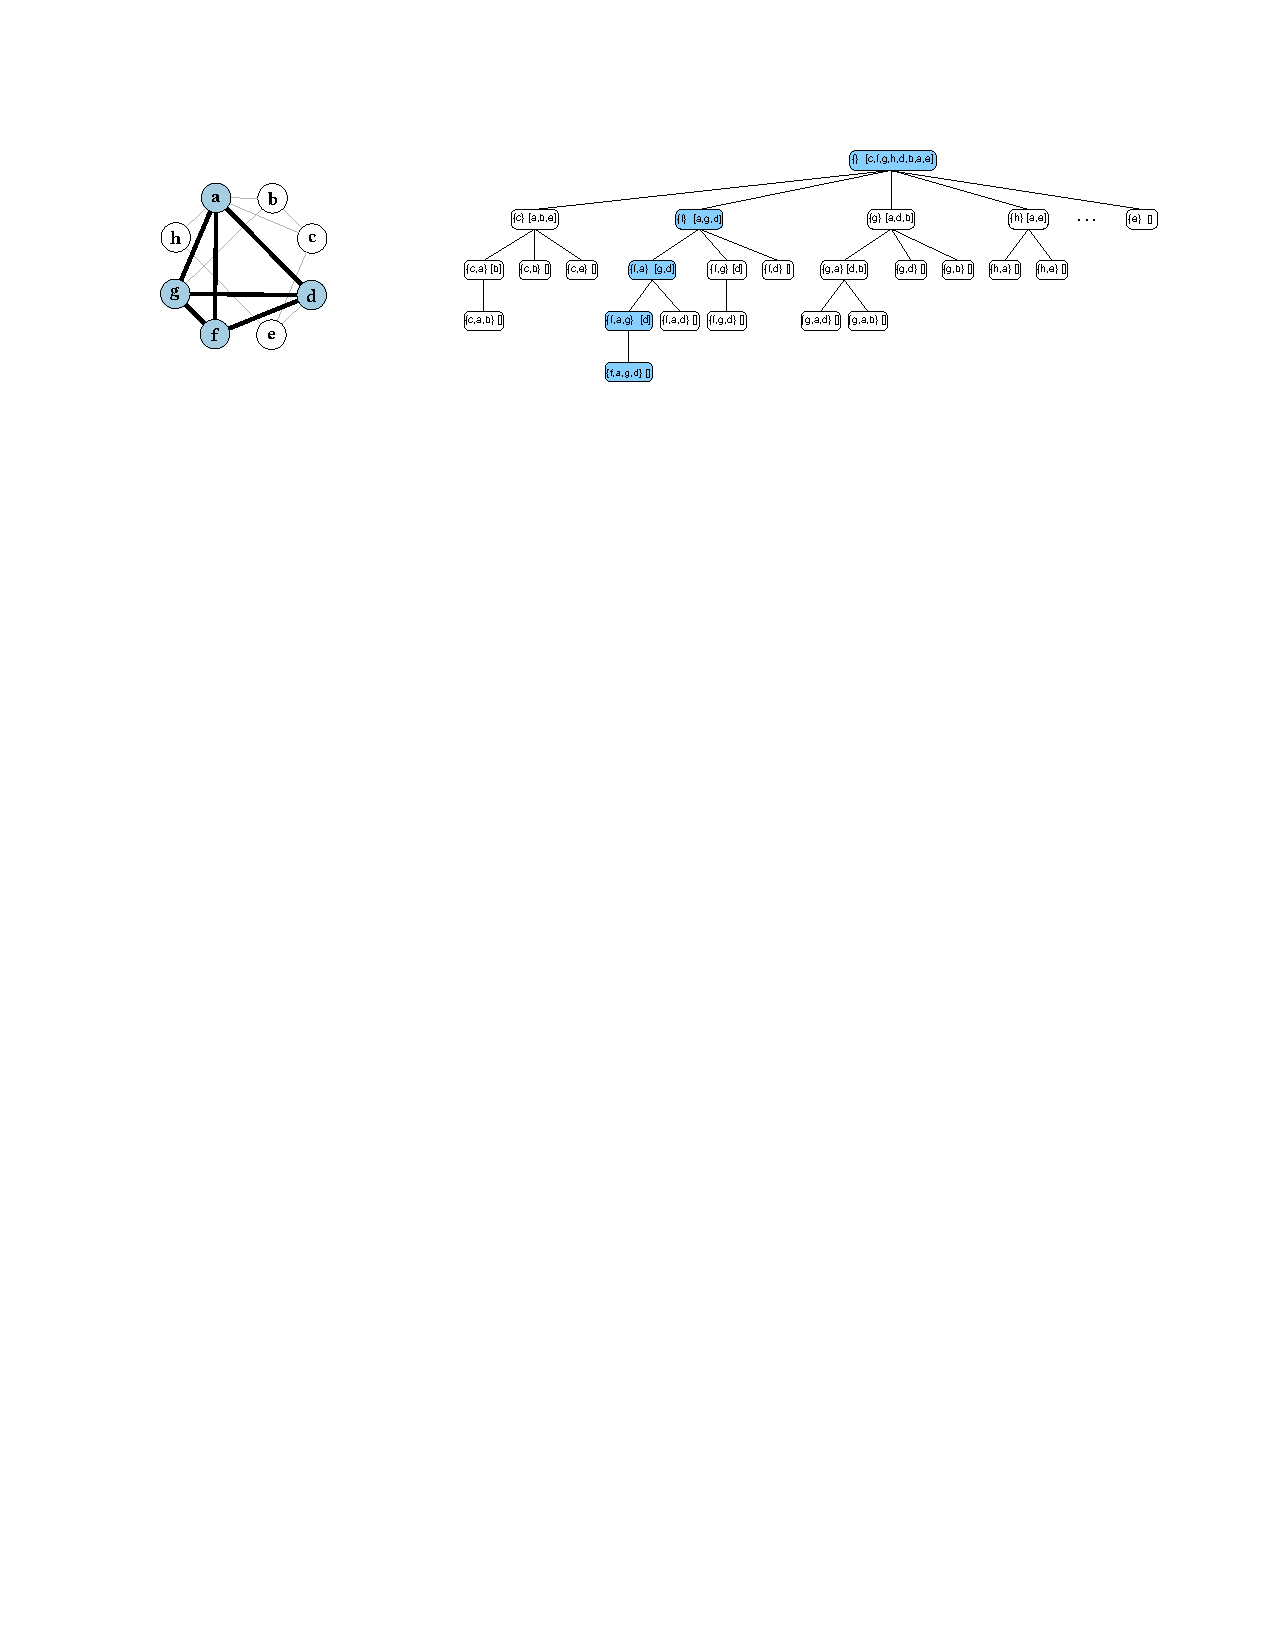
\includegraphics[width=0.98\textwidth]{images/yewpar_maxclique.pdf} % 插入图片,设置图片宽度为文本宽度的80%
    \caption{Maximum clique instance in YewPar. Input graph with clique \{a,d,f,д\} to the left and corresponding search tree to the right.
        Each tree node displays the current clique and a list of candidate vertices (in heuristic order) to extend that clique.\cite{10.1145/3332466.3374537}} % 提供图片的注解
    \label{fig:yewpar_maxclique} % 为图片提供一个标签,以便在文档的其他地方引用
\end{figure}
\FloatBarrier

而YewPar是一个专为组合搜索设计的并行框架.
它提供了一套强大的工具和策略,允许开发者轻松地并行化他们的搜索算法.
YewPar的主要特点是其灵活性和可扩展性,
使其能够应对各种复杂的搜索场景.
其中,workstealing是YewPar中用于任务调度的核心策略,
它允许处理器在本地任务队列为空时从其他处理器窃取任务,确保所有处理器都能保持忙碌,从而提高整体性能。

\subsubsection{Performance Anomalies}
\label{sec:performance_anomalies}
搜索算法依赖于排序启发式方法尽早找到有用的节点,
例如决策问题中的目标节点,
或者分支限界优化问题中的一个强约束节点。为了利用这些启发式方法,
搜索按从左到右的顺序进行(在树的所有深度上).
因此,访问节点的顺序搜索具有关于搜索树的完整信息,
例如来自它左侧的所有节点的当前最佳解,并且搜索是确定性的。
并行搜索在没有完整的左侧信息的情况下推测性地搜索子树,
并可能从从右到左的信息流中受益。
但是,这种推测意味着并行搜索可能比相同的顺序搜索执行更多的工作。
因此,并行搜索因性能异常而臭名昭著\cite{10.1007/3-540-60321-2_29}.
有害的异常是当w个工作线程上的运行时间超过w-1个工作线程时发生的。
在这里,额外的工作可能超过额外计算资源的好处,
或者额外的计算资源可能会破坏搜索启发式方法。
加速异常是超线性的加速,通常是由于从右到左的知识流动,
通过允许比顺序搜索中更多的修剪来减少总体工作量。
异常的存在使得推理搜索应用的并行性能变得困难。
Yew-Par旨在避免有害的异常,同时允许加速异常;
\cite{ARCHIBALD201892}报告了一个专门的搜索框架,该框架仔细控制异常以提供可复制的性能保证。

\subsection{为什么要在YewPar中设计并使用新的workstealing策略}

YewPar采用workstealing作为其核心的分布式并行化调度策略,
但其采用的是偏随机窃取的策略\cite{archibald2019yewpar},
空闲的worker会随机尝试窃取其它节点的任务直到获取到有效任务后锁定该节点窃取,
直至不再能从该节点再窃取到任务后再重新随机选择节点进行窃取,
这种方法可能导致不必要的开销和计算资源的空闲,
尤其是在不均匀的任务分布和各节点具有不均衡的计算资源下.
考虑到组合搜索的特性,
各节点的任务数量可能存在较大差异,
任务之间也可能存在巨大的执行时间差异,
这使得随机窃取策略会更大概率导致空闲worker有较长的饥饿时间,
并不是最优选择。

为了更好地利用各节点的各个核心的计算能力并减少不必要的通信开销,
YewPar需要一种更加智能的workstealing策略。
基于各节点性能的新的Performance-Driven Workstealing Policy正是为了解决这一问题而提出的。
通过低成本评估每个节点的性能如平均任务执行时间等,
新策略采用根据各性能参数设计的窃取算法可以更精确地动态刷新最优窃取目标,
提高整体性能。



%%%%%%%%%%%%%%%%%%%%%%%%%%%%%%%%%%%%%%%%%%%%%%%%%%%%%%%%%%%%%%%%%%%
\chapter{Design and implementation}\label{design}

\section{总体设计}

本文设计的Performance-Driven Workstealing Policy框架包含了:
\begin{itemize}
    \item Scheduler Channel(主要负责监测与统计与传输节点所有workers的负载状态).
    \item Performance Monitor(主要负责统计各项性能数据与发送各项处理后的本地性能数据,并计算和缓存最优窃取目标节点的id).
    \item Performance Policy(在本地任务池无任务时,主要负责从Performance Monitor获取最优窃取目标)
\end{itemize}

组件之间的关系大致如\cref{fig:overall_architecture}所示.
\begin{figure}[h] % 'h'表示图片尽量在当前位置
    \centering % 让图片居中显示
    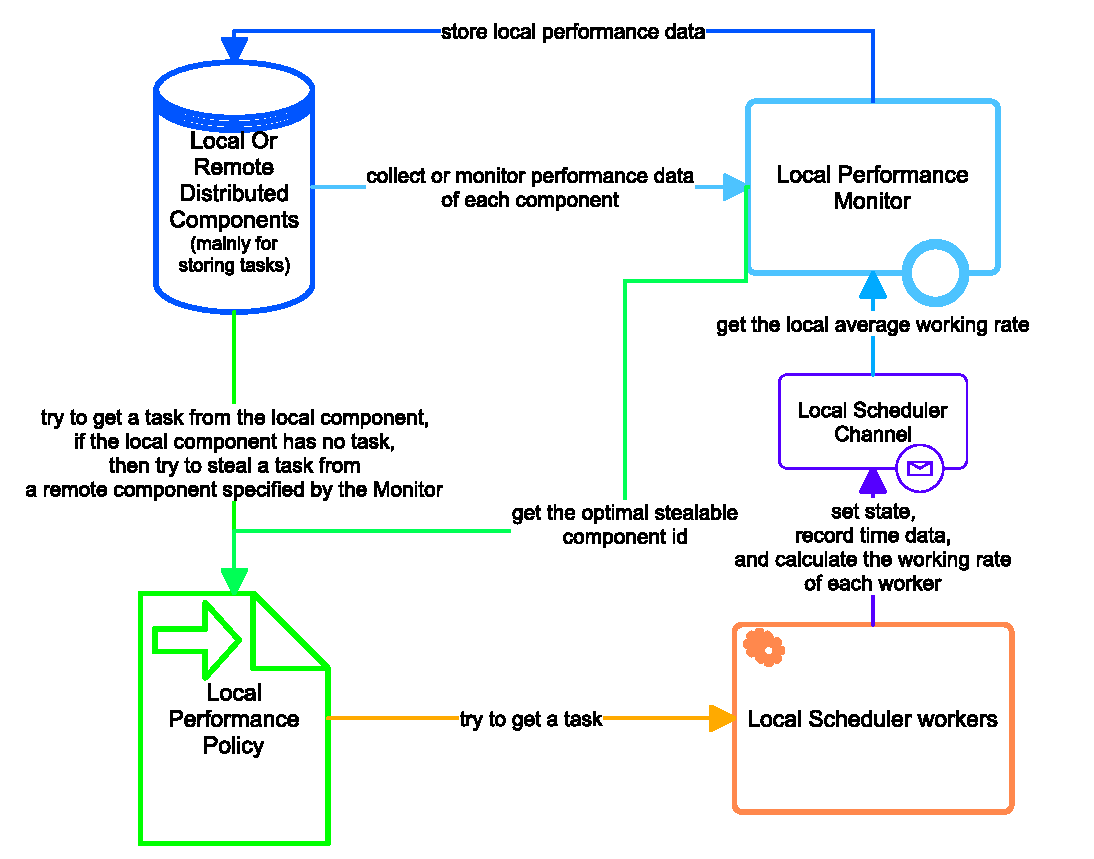
\includegraphics[width=0.9\textwidth]{images/overall_architecture.pdf} % 插入图片,设置图片宽度为文本宽度的80%
    \caption{Performance-Driven Workstealing Policy Architecture} % 提供图片的注解
    \label{fig:overall_architecture} % 为图片提供一个标签,以便在文档的其他地方引用
\end{figure}
\FloatBarrier

其中Performance Monitor主要负责各项性能数据的统计和传输,并计算和缓存最优窃取目标节点的id;
distributed component负责存储可供远程和本地访问的任务池和性能等数据,
通过hpx框架的action提供访问与改写操作;
Scheduler Channel提供接口让workers能更新自己当前负载状态并计算自己的负载数据,
workers负责从Performance Policy获取可执行的任务;
Performance Policy负责调取本地任务池任务或者从Performance Monitor获取最优窃取目标节点后窃取其任务池任务.

%%%%%%%%%%%%%%%%%%%%%%%%%%%%%%%%%%%%%%%%%%%%%%%%%%%%%%%%%%%%%%%%%%%

\section{性能数据收集与传输}
数据收集包含三部分:各节点负载情况,各节点剩余任务量,各节点获取任务池任务的耗时.
这三个参数将会为后续的最优窃取目标计算提供有力的数据支持.
同时,为了保障能以较低成本收集到更有效的数据,本文对三部分都进行了仔细的设计与优化.

\subsection{节点所有worker的负载情况}
首先,YewPar的System Stack大致如
\cref{fig:yewpar_system_stack}
\cite{10.1007/978-3-030-29400-7_14}
所示.

\begin{figure}[h] % 'h'表示图片尽量在当前位置
    \centering % 让图片居中显示
    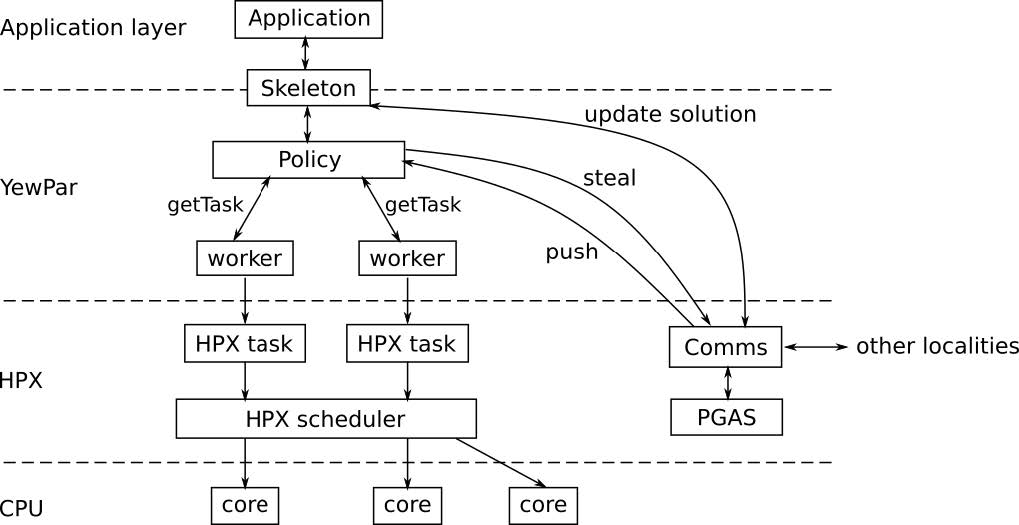
\includegraphics[width=0.9\textwidth]{images/YewPar_System_Stack.jpg} % 插入图片,设置图片宽度为文本宽度的80%
    \caption{YewPar System Stack} % 提供图片的注解
    \label{fig:yewpar_system_stack} % 为图片提供一个标签,以便在文档的其他地方引用
\end{figure}
\FloatBarrier

其中Policy负责被worker调用时,
通过尝试图从本地池获取任务或从其它节点任务池偷取任务,
而真正负责执行任务的是YewPar的各个worker,
所以如果想要不依赖系统底层函数获得各节点的负载情况,
比较简单好用的方法就是去获取各节点的workers的负载情况.
本文对YewPar框架下的worker的工作流程进行了分析,如\cref{fig:period_of_worker}

\begin{figure}[h]
    \centering % 让图片居中显示
    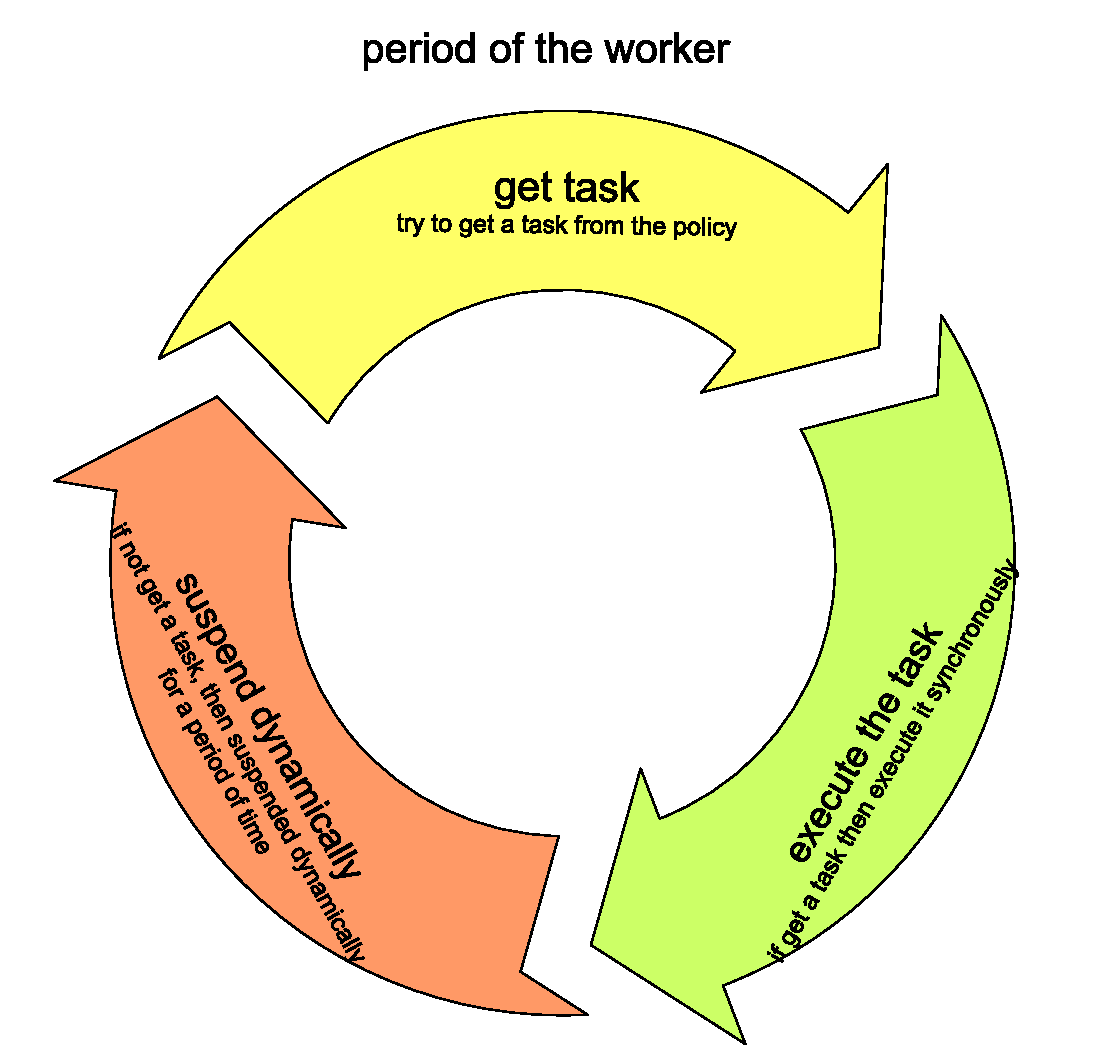
\includegraphics[width=0.7\textwidth]{images/period_of_worker.pdf} % 插入图片,设置图片宽度为文本宽度的80%
    \caption{period of the worker} % 提供图片的注解
    \label{fig:period_of_worker} % 为图片提供一个标签,以便在文档的其他地方引用
\end{figure}
\FloatBarrier

可以看出每个worker从创建到销毁之间,
它的生命周期都处在一个循环中,其中包含了三个可能的阶段:
\begin{enumerate}
    \item 调用Policy的getWork函数获取任务;
    \item 如果获取到任务则执行该任务;
    \item 如果没有获取到任务则休眠一段时间,这段时间随着没有获取到任务的次数的增加而增加,当再次获取到任务时则时间重置.
\end{enumerate}

这三个阶段中,第一阶段是每次循环都会经历的阶段,
而第二阶段和第三阶段则是互斥关系,每次循环只会经历其中一个阶段.

如果需要分析worker的真实负载情况,
就需要以第二阶段为核心进行统计,
因为第二个阶段是worker真正执行任务的阶段,
它所消耗的时间是worker执行任务的时间,也就是有效的负载时间,
而其它阶段所消耗的时间则可以归类为worker的空闲时间,
因为这段时间并没有执行任何任务,也就是无效的负载时间.

由于原先一个周期未必能经历第二阶段,
所以为了避免更新无效数据,
本文对worker的生命周期判定进行了重定义,
以一个任务的执行完毕为一个新周期的开始,
以一个任务的开始为一个周期的结束,
这样便能保证每个周期都能经历第二阶段,也就是执行任务的阶段.

在此理论基础上,本文设计了如\cref{fig:worker_collect_calculate}的一套完整的数据收集方案,

\begin{figure}[h]
    \centering % 让图片居中显示
    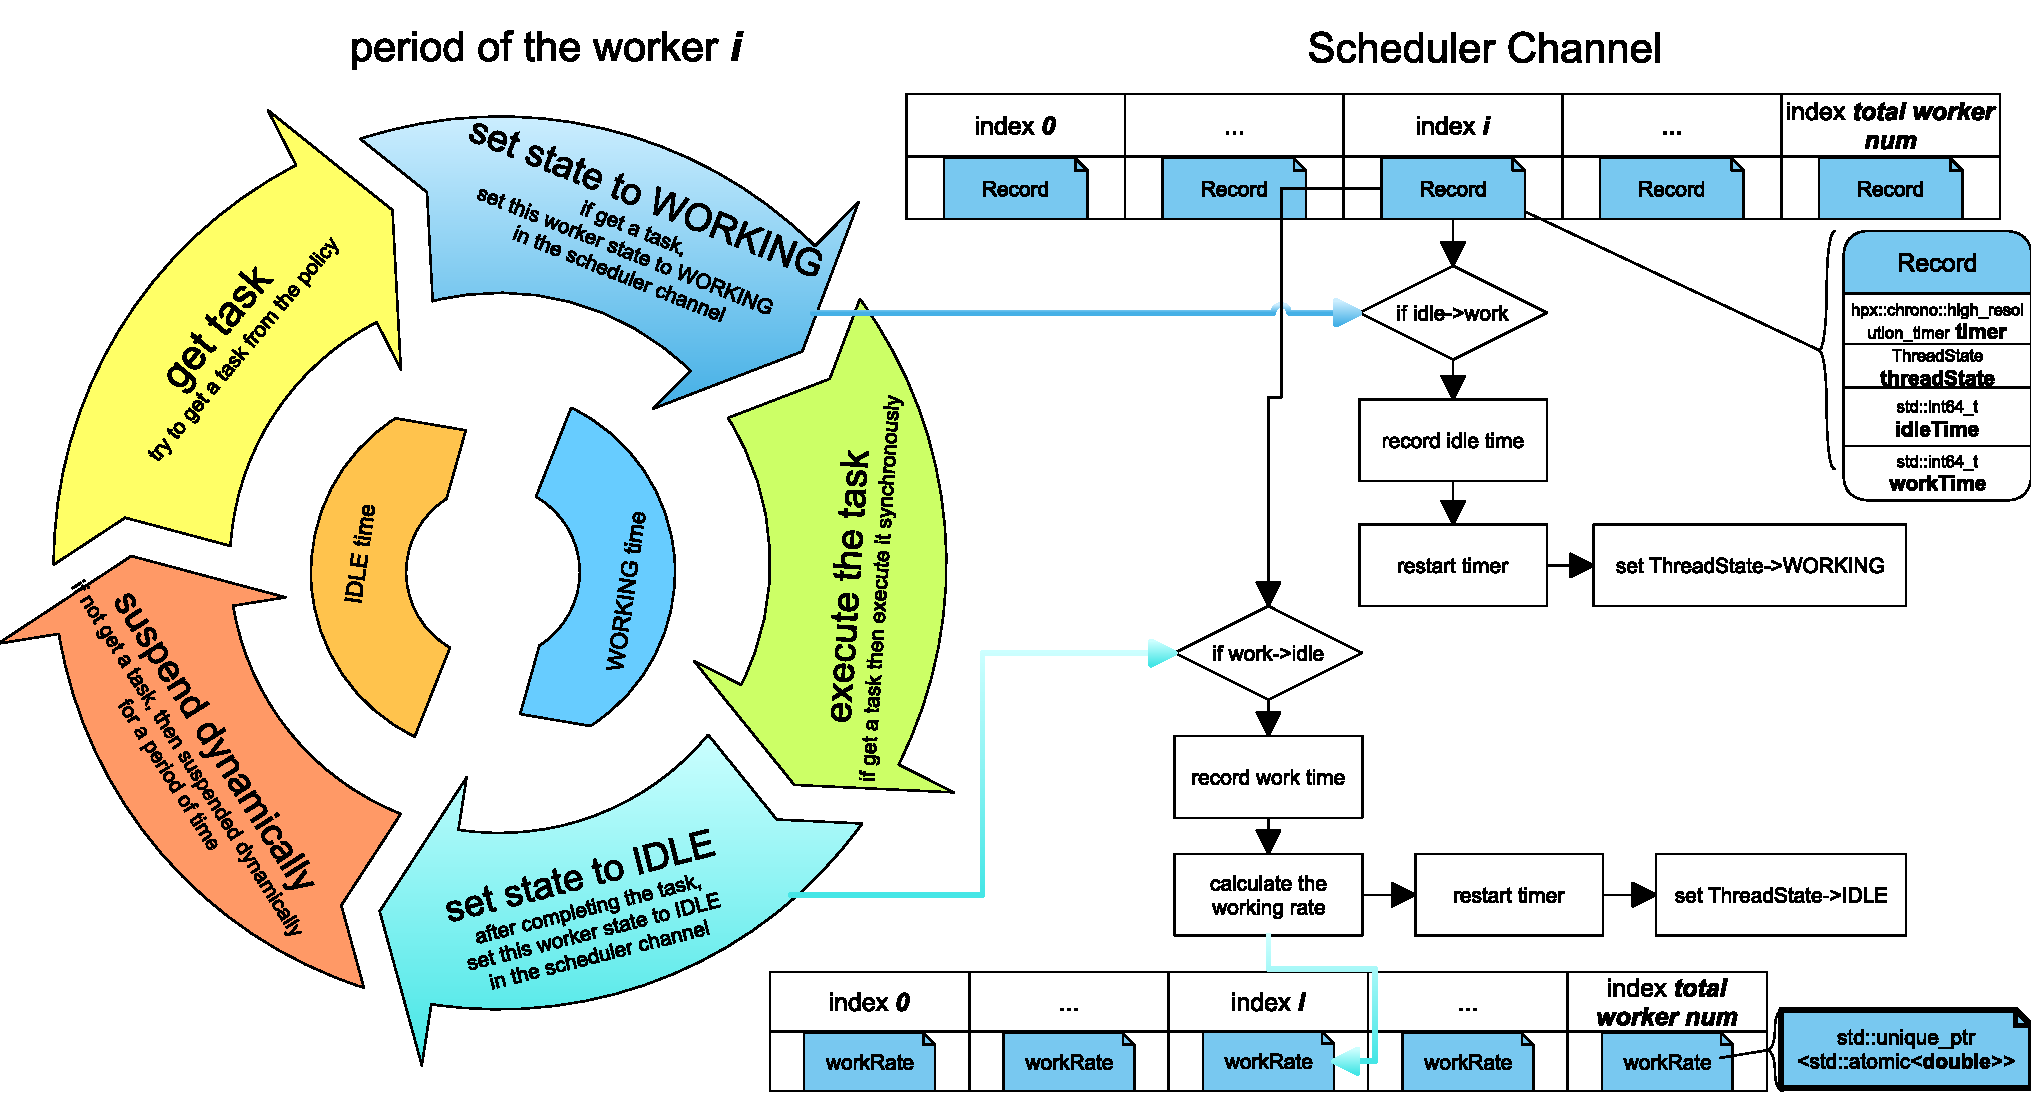
\includegraphics[width=1.0\textwidth]{images/worker_collect_calculate.pdf} % 插入图片,设置图片宽度为文本宽度的80%
    \caption{collect worker state to calculate the workload} % 提供图片的注解
    \label{fig:worker_collect_calculate} % 为图片提供一个标签,以便在文档的其他地方引用
\end{figure}
\FloatBarrier

通过在任务执行的开始和结束位置插入探测代码(一旦执行,即暂停当前流程,转而执行探测相关的操作),
worker可以在任务执行前后更新其状态到Scheduler Channel模块(一个专用于状态传输的channel).
这样,worker能够实时计算并更新其负载数据,为Performance Monitor提供所需数据进行进一步计算。

"Scheduler Channel使用了特定的数据结构来统计数据,
为了避免使用锁带来的开销,
它采纳了无锁化的设计策略\cref{survey_lock}.
这种设计旨在减少workers间在统计负载数据时的竞争.

该数据结构主要由两组数组构成,每组的长度均等于本地workers的数量:
\begin{enumerate}
    \item Record数组: 这组数组存储特定的Record数据结构,每个Record包括:
          \begin{itemize}
              \item 一个计时器timer
              \item 当前的状态threadState
              \item 当前周期的空闲时间idleTime
              \item 当前周期的工作时间workTime
          \end{itemize}
          这样的设计允许workers记录自己在各种状态下的持续时间.
          由于每个worker都对应一个独立的record,所以可以避免使用锁,从而提高性能。
    \item workRate数组: 这组数组存储了通过特定算法计算出的worker的负载率数据。
          每个workRate是一个被unique\_ptr包装的原子double类型。
          虽然worker和Monitor可能会同时访问这些数据,
          但由于workRate是基础数据类型,
          所以采用原子类型可以确保在无锁环境下数据的正确性。
\end{enumerate}

这里收集负载数据大致由两种流程组成:
\begin{itemize}
    \item 在"set state to WORKING"阶段,worker主要在channel更新自己这轮周期的空闲时间,并更改状态为WORKING;
    \item 在"set state to IDLE"阶段,worker主要在channel更新自己这轮周期的工作时间,
          并根据空闲与工作时间与历史workRate数据计算出当前的workRate,并更改状态为IDLE.
\end{itemize}

在"set state to IDLE"阶段,计算最新的workRate的算法如\cref{eq:workrate}所示:

\begin{align}
    \text{workRate} & = \left( \ln\left( 2.72 + \frac{\text{workTime}}{\text{workTime} + \text{idleTime}} \right) \right. \notag   \\
                    & \qquad \times \left. \ln\left( 2.72 + (\text{workTime} + \text{idleTime}) \right) \times 0.65 \right) \notag \\
                    & \qquad + \text{workRate} \times 0.35 \label{eq:workrate}
\end{align}

公式目的是为了计算当前worker是否繁忙和计算速度是否较慢,主要分为三部分:
\begin{enumerate}
    \item $\ln\left( 2.72 + \frac{\text{workTime}}{\text{workTime} + \text{idleTime}} \right)$,
          这是由于在每个周期中,如果WORKING状态的持续时间相对IDLE状态的持续时间比值越大,
          则说明当前任务量较大或者任务较为复杂,所以相对需要更多的时间来执行任务,
          相反则说明当前worker的任务饥饿时间较长,浪费了大量时间在试探窃取任务等无效负载的时间上.
          同时因为时间数据采用微秒为单位,数据较大导致数据波动也大,
          为了避免数据过于敏感,所以采用了对数函数来降低数据的敏感度,
          使用了$(2.72+...)$是为了保证结果永远为正数.

    \item $\ln\left( 2.72 + (\text{workTime} + \text{idleTime}) \right)$,
          这是考虑到之前比值的结果并不能很好地反应出当前worker的运行速度,
          可能它处在任务量较小但是由于运行速度慢,所以实际负载还是比较大的情况,
          所以需要计算当前周期的总耗时,
          将总耗时乘以之前计算出的比值,就可以得到当前周期的一个实际负载情况,
          同时由于是微秒级别的时间数据,所以也采用了对数函数来降低数据的敏感度.

    \item $(... \times 0.65 +\text{workRate} \times 0.35)$,
          这是由于刷新数据可能是间隔一段时间再刷新,
          所以保留历史负载数据作为参考防止因为短期波动导致对当前worker的负载情况判断失误是很有必要的,
          而当前记录负载率的数据结构为了节省内存空间的消耗,
          未设置例如数组或其它结构保存历史负载数据,
          所以在节省空间的同时为了节省计算时间,
          这里通过采用了一种称为指数平滑\cite{GARDNER2006637}的简单算法,
          通过给与历史workRate数据一定的系数和当前workRate数据一定的系数后相加,
          来让workRate数据既反应了当前的负载情况,也保留了一定的历史数据参考,
          而系数0.65和0.35则是为了更好地反应当前的负载变化情况,
          所以设置当前workRate的系数偏大,
          而历史workRate的系数偏小,
          之后经过多次在集群环境的测试后得出的一个较为合理的系数,
          从而使得数据更加平滑和更具参考价值.
\end{enumerate}

最终,计算出的各个worker的workRate数据会相加后除以worker的数量算出平均负载数据,
处理后的数据只是一个double类型的数据,非常轻量,
这时再递交给Performance Monitor,
让它将本地workRate数据提交给local distributed component以方便其它节点进行快速查询.

\subsection{各节点剩余任务量与通讯延迟时间收集}\label{collect_tesks_delay}

性能数据还需要对各节点剩余任务量和获取花费时间进行收集,
具体实现如\cref{fig:tasks_detection}所示.

\begin{figure}[h]
    \centering % 让图片居中显示
    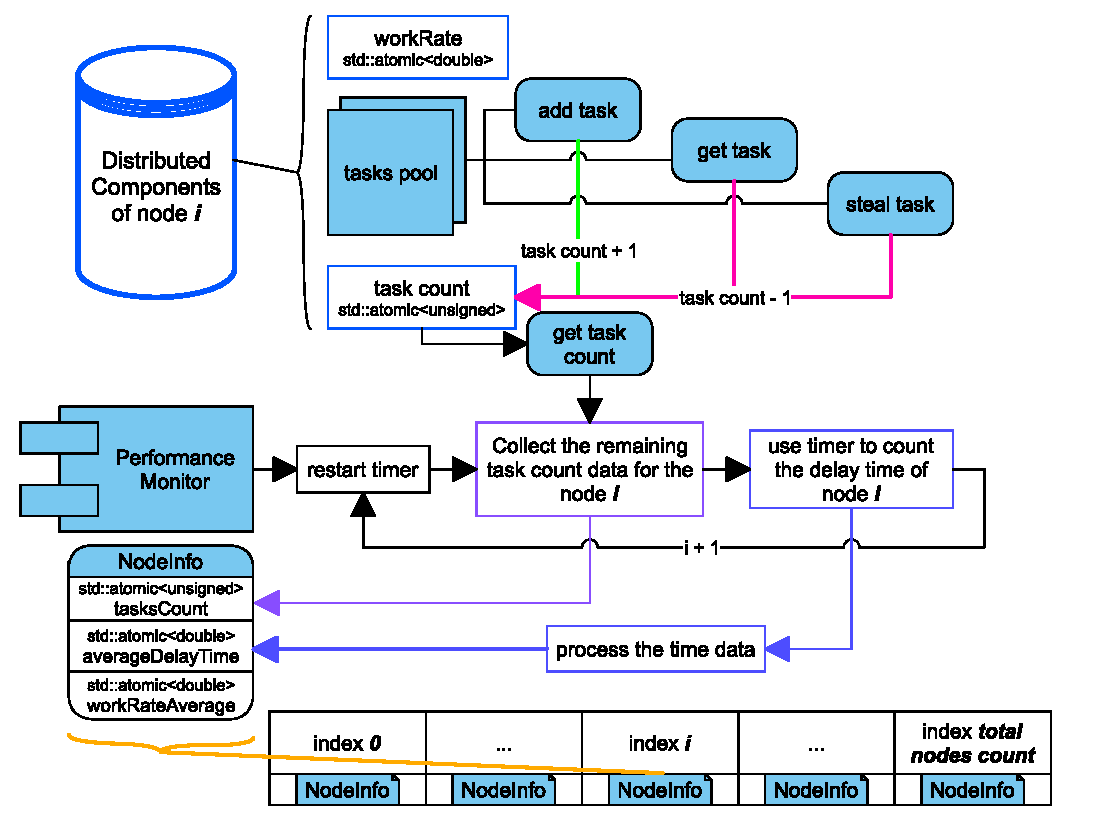
\includegraphics[width=0.98\textwidth]{images/tasks_detection.pdf} % 插入图片,设置图片宽度为文本宽度的80%
    \caption{collect tasks count and delay time} % 提供图片的注解
    \label{fig:tasks_detection} % 为图片提供一个标签,以便在文档的其他地方引用
\end{figure}
\FloatBarrier

在hpx分布式组件中包含了任务池与剩余任务数量,
其中剩余任务数量是因为本文的框架需要而后期添加的,采用轻量的原子类型保障数据安全,
原先任务池有三种分布式操作可以更改任务池:
添加任务,获取任务与窃取任务.
所以为了剩余任务数量数据的正确,
在调用这三种操作时会对剩余任务数进行如\cref{fig:tasks_detection}所示地更新.
在每个节点的Performance Monitor中,
会定时遍历并调用各节点的distributed component的get\_task\_count接口以获取节点的剩余任务数.

而为了统计本地节点与各节点的通讯延迟时间,
也就是为了统计各节点的分布式组件间的数据获取所需时间,
而之前获取各节点的剩余任务数时,
正好是获取分布式组件的数据的操作,
所以通过计算获取各节点的剩余任务数的耗时,
也就在不额外占用通讯IO的同时统计出了本地节点与各节点的通讯延迟时间.

补充一点,这里通讯延迟时间也稍微反应了节点线程池的繁忙程度,
因为任务数量是采用原子类型,
那么当任务池繁忙时,
往往会因为小幅度阻塞其它修改操作导致获取任务数的耗时增加;

由于获取的通讯延迟时间是一项时间数据,可能具有较大的数值与波动,所以需要处理后再存储,
处理公式为
\begin{align}
    \text{averageDelayTime}_i & = \ln\left(2.72 + \text{delayTime} \times \text{worker\_count}\right) \times 0.65 \notag               \\
                              & + \text{nodeInfoVector}[i]\texttt{->}\text{averageDelayTime} \times 0.35   \label{eq:averageDelayTime}
\end{align}
其中$i$为各节点编号,
由于hpx框架下各节点的编号不变,
所以可以作为数组的索引方便定位各节点,
$\text{delayTime}$为通讯延迟时间,$\text{worker\_count}$为节点worker数量,
公式首先通过将延迟时间乘以本地的worker数量来反应节点总体的通讯耗时,
再同时参考\cref{eq:workrate}也通过对数函数与指数平滑来降低数据的敏感度,
并保留了部分历史数据的影响,
使数据更加平滑和更具参考价值.

在处理后会将数据进行存储,
存储的数据结构也采用了无锁化设计,
如\cref{fig:tasks_detection}所示是一个长度为节点总数的数组,
index编号对应各节点编号,
数组中存储着一个称为NodeInfo的数据结构,
其中包含着编号对应节点的原子类型的节点负载率,剩余任务数与平均通讯延迟时间,

\section{最优窃取目标计算与缓存}

在Performance Monitor通过性能收集机制获得了包括
各节点负载情况,各节点剩余任务量,各节点通讯延迟等性能数据后,
Performance Monitor会通过这些数据计算出最优窃取目标节点,
并将节点的id缓存起来以供后续Performance Policy获取.
其整体流程如\cref{fig:refresh_target}所示.

\begin{figure}[h]
    \centering % 让图片居中显示
    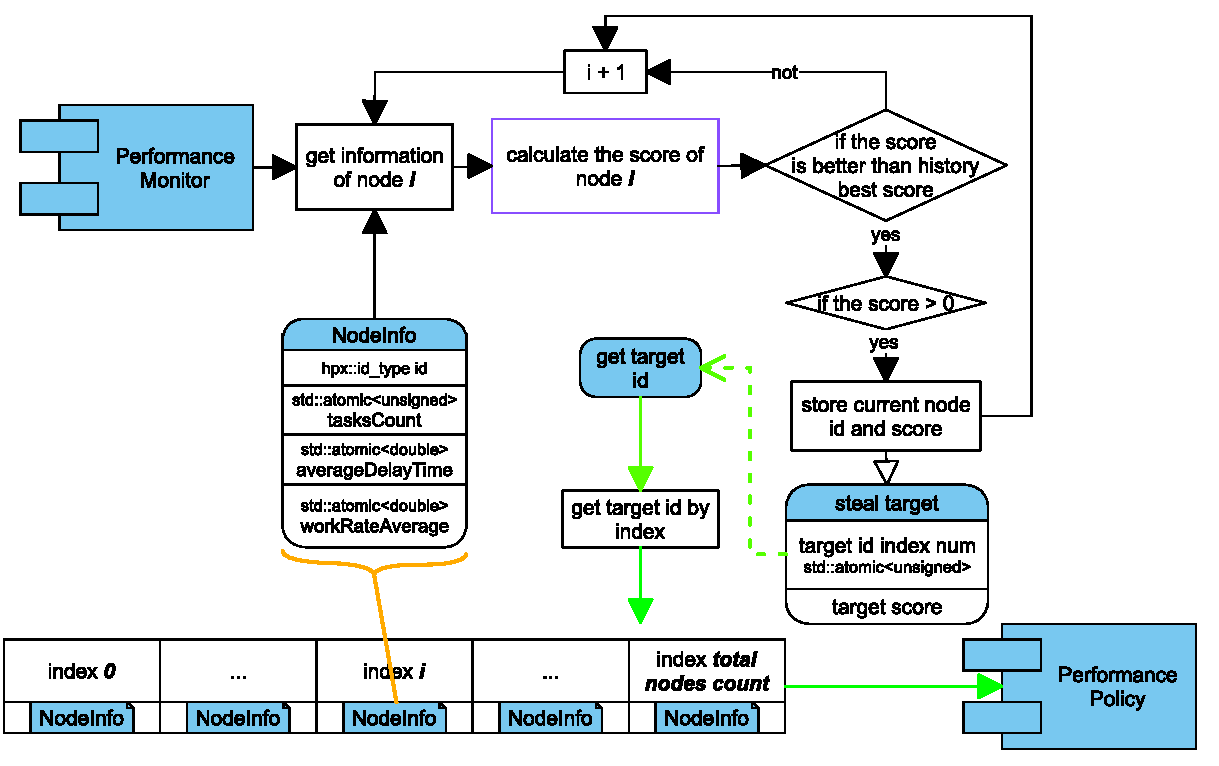
\includegraphics[width=1\textwidth]{images/refresh_target.pdf} % 插入图片,设置图片宽度为文本宽度的80%
    \caption{refresh the optimal steal target} % 提供图片的注解
    \label{fig:refresh_target} % 为图片提供一个标签,以便在文档的其他地方引用
\end{figure}
\FloatBarrier

这里数组的数据结构在之前\cref{collect_tesks_delay}进行过介绍.

这套流程首先通过遍历各节点的NodeInfo数据结构中性能数据,来计算各节点的steal-worthiness score,
得分越高则说明越值得窃取,
其计算公式为
\begin{align}
    \text{score}_i & = \max\left(\text{nodeInfoVector}[i]\texttt{->}\text{workRateAverage}, 0.0001 \right) \notag \\
                   & \quad\times \text{nodeInfoVector}[i]\texttt{->}\text{tasksCount} \notag                      \\
                   & \quad - \text{nodeInfoVector}[i]\texttt{->}\text{averageDelayTime} \label{eq:score}
\end{align}

公式的核心思想是尽量减少具有最大负载量的节点的任务同时,
一定程度减少浪费在窃取任务上的时间.
其分为以下几个部分:
\begin{enumerate}
    \item 通过$\max\left(\text{nodeInfoVector}[i]\texttt{->}\text{workRateAverage}, 0.0001 \right)$
          来避免过小的无意义数据对计算的干扰.
    \item 再通过$\times \text{nodeInfoVector}[i]\texttt{->}\text{tasksCount}$
          也就是该节点的负载率与剩余任务数的乘积,
          来预估该节点的总共负载量.
    \item 最后通过$- \text{nodeInfoVector}[i]\texttt{->}\text{averageDelayTime}$
          来减去一定的通讯延迟,
          避免窃取任务时浪费过多时间.
\end{enumerate}

最终得到的结果越大则说明该节点越值得窃取,
因为它的负载量较大,需要比其它节点更长的时间去处理剩余任务,
同时它的通讯延迟也较小,窃取任务时浪费的时间也较少.

在遍历完所有节点后,一般会得到一个最优的节点目标编号索引,
会将这个最优的节点目标编号索引数进行缓存,
当Performance Policy需要获取最优窃取目标的$id\_type$时,
会通过提供的查询接口,
通过索引再去节点数组里获取最优窃取目标节点的$id\_type$.
这样设计的一个原因是由于hpx的$id\_type$类型非基本数据类型,
不能将其原子化,
而其对应的数组索引编号数字是可以原子化的,
为了保持整体的无锁化设计避免因长时间阻塞导致计算资源浪费,
通过在刷新阶段只变更存储的索引数字,
而在查询阶段只通过索引数字去读取对应的$id\_type$,
这样所有的$id\_type$只会被读取而不会被修改,
保障了无锁化下的数据安全.

在判断选出的最优窃取目标是否具有窃取价值,这主要从两个方面判断:
\begin{itemize}
    \item 窃取目标是否已无剩余任务可窃取.
    \item 窃取的成本是否高过了收益,
          即在窃取任务消耗的时间大于了帮助目标节点完成任务所节省的时间,
\end{itemize}
而这种情况下score往往会小于或者等于0,
所以设置了额外的判断条件,在score小于或者等于0的情况下不会缓存最优窃取目标,
此时worker在Performance Policy的策略下会再次尝试获取最优窃取目标,
失败后进入短暂的休眠避免过于频繁的尝试导致计算资源的浪费.

\section{Refresh data and provide tasks mechanism}

在建立了一套从数据收集到计算最优窃取目标和缓存最优窃取目标的机制后,
我们还需要解决的问题,就是以何种频率去刷新各项数据.
虽然每一次刷新数据的开销都是相对很小的,
但是YewPar的worker数量会尽量占满本地的计算资源,
那么当worker繁忙时,过于频繁的刷新会导致worker的工作被打断,
从而一定程度影响YewPar的性能.
但是如果刷新的频率过低,则会导致数据的可靠性降低,
因为数据的实时性降低,
提供给其它节点的数据和缓存的其它节点数据都将不够准确,
甚至可能导致窃取到其它任务饥饿的节点,加剧不均衡的情况.

为解决这一问题,本文设计了一种双向动态刷新的刷新机制,
它由两种刷新方式组成,
一种是自动动态刷新任务方式,另一种是通过Performance Policy进行辅助刷新方式.
大致流程如\cref{fig:refresh_provide}所示.

\begin{figure}[h]
    \centering % 让图片居中显示
    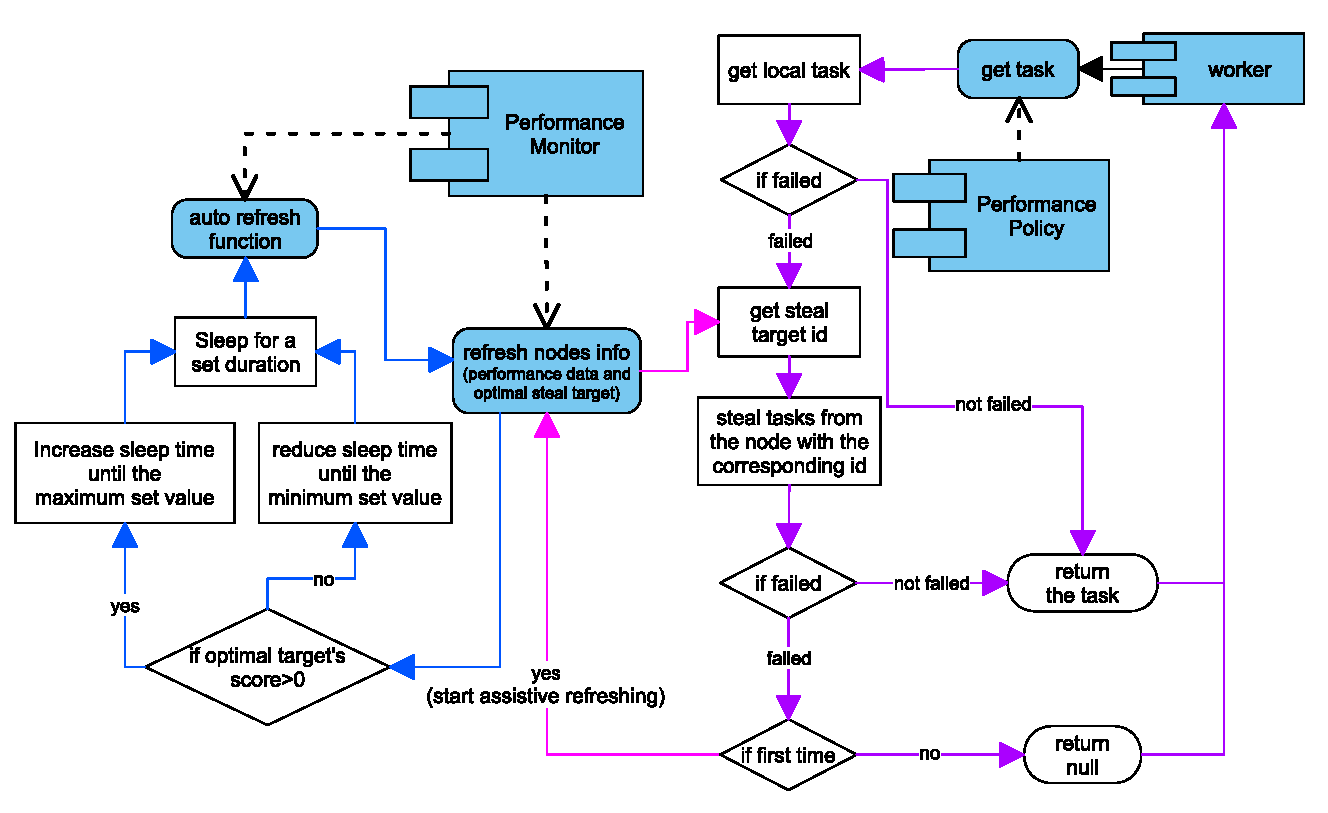
\includegraphics[width=0.98\textwidth]{images/refresh.pdf} % 插入图片,设置图片宽度为文本宽度的80%
    \caption{refresh data and provide tasks mechanism} % 提供图片的注解
    \label{fig:refresh_provide} % 为图片提供一个标签,以便在文档的其他地方引用
\end{figure}
\FloatBarrier

在图的左侧,是在Performance Monitor中部署的自动动态刷新任务,
它的本质上是一个循环,在每次刷新数据后都会根据刷新结果动态调整下一次刷新的时间,
如果刷新数据的结果不理想,
则说明当前很可能仍有worker处在饥饿的状态,
则会大幅缩短下一次刷新的时间;
但如果刷新数据的结果符合预期,
则说明workers很可能都会成功获取到任务进行执行,
所以会逐渐增加下一次刷新的时间,
避免频繁的刷新影响worker的计算性能.
而刷新数据的结果是否理想目前主要通过score进行判断,
目前的算法是如果score小于等于0则说明不理想,
因为根据\cref{eq:score}大概率是任务池任务数过少或者获取任务耗时过长导致的,
这种情况下,很可能会导致窃取的成本高于收益,
比如窃取时目标节点已无任务可窃取,
或者窃取的通讯延迟时间和本地执行时间相加不如远程节点自己执行完剩余任务的时间短等.
这里需要说明的是,虽然动态调整时间在实践中收益明显,
但是仍需要设置上下限,
因为如果不设置上限很可能导致由于落后的数据导致缓存了的错误窃取目标,
而如果不设置下限则会导致频繁的刷新影响了其它仍有任务执行的worker的性能或者影响系统底层的调度,
而如何界定这个上下限的值通过后续的多次实验,
发现在一定范围内既能达到对系统性能影响较低,又能保障数据的相对实时性,
而之前的通过加入了指数平滑等算法设计,
通过一定程度保留了历史数据的影响,
导致了数据即使有一定的延迟也能较为准确的反应各节点的综合情况.

而上述设计仍有不足之处与优化的空间,
所以还设计了如\cref{fig:refresh_provide}的右侧所示的一种通过Performance Policy进行辅助刷新的机制,
Performance Policy的本质是获取任务的一个策略,
它会优先获取本地的任务进行执行,
因为如果本地有任务的话会让worker更快地获取到任务并执行,
避免计算资源的浪费,
但是如果本地获取不到任务,
则会优先对Performance Monitor的最优窃取目标的id缓存进行查询,
通过获取的id对远程对应节点的任务池进行窃取,
这样大概率会窃取到有效的任务返回给worker进行执行,
从而尽可能避免worker的饥饿状态,
但是当各节点任务剩余数量都很少等情况下,
有小概率会无法窃取到任务,
这种在初期刚开始逐步生成任务,
或者在各节点都快执行完任务且很少有新任务加入时的情况下会出现的较多.
而自动刷新机制有可能此时在休眠状态无法及时调整刷新时间,
此时被woker调用的Performance Policy就会担任辅助刷新的作用,
主动去同步执行刷新数据的任务,
因为一方面不刷新数据则大概率这个worker还是会处于饥饿状态,
另一方面刷新数据时会占用这个worker的计算资源,而不会去影响其它worker,
但是如果获取到有效的窃取目标则会给自己和其它worker都带来收益,
当刷新数据完成后会再次尝试根据新的目标窃取一次任务,
如果还是失败则大概率说明当前各节点都很少有任务,
为了避免通讯等资源的占用,此时会返回空数据让这个worker进入休眠周期避免资源的占用.

而在实际实践中也发现两套机制互相配合能够很好地提升系统的性能.

%%%%%%%%%%%%%%%%%%%%%%%%%%%%%%%%%%%%%%%%%%%%%%%%%%%%%%%%%%%%%%%%%%%
\chapter{Evaluation}

\section{Search Applications}

我们对YewPar原有的两种搜索类型的代表性搜索应用和代表性样本上评估改进workstealing策略后的性能,
如下所示.

\begin{itemize}
    \item Enumeration:
          非平衡树搜索(UTS)根据给定的分支因子、深度和随机种子动态地构建合成的不规则树工作负载\cite{olivier2006uts}.
          数字半群(NS)计算具有特定属数的数字半群有多少\cite{fromentin2016exploring}.
          数字半群S是一个包含0且在加法下封闭的自然数的余集;
          S的属数是其补数的大小.
    \item Optimisation:
          最大团(MaxClique)找到给定图中的最大团,
          即最大的两两相邻顶点的集合。
          0/1背包问题确定将每个具有利润和重量的物品放入容器中的最佳组合,
          使得在给定的重量限制下利润最大化。旅行商问题(TSP)找到N个城市的最短循环之旅。
\end{itemize}

为了控制变量,
评估使用的应用程序maxclique-16和NS-hivert是YewPar的hpx1.8分支自带的应用程序,
并未对其进行改动,
但运行时窃取策略分别使用了改动后的Performance-Driven Workstealing Policy
和原版的hpx1.8分支的DepthPool Policy以进行对比.
其中MaxClique\cite{mccreesh2013multithreading}、
NS\cite{fromentin2016exploring}的基线实现使用了公开的先进算法.
这些顺序的C++实现是由领域专家提供的.
关于应用程序和实例的完整描述在\cite{archibald2018}中.

对maxclique-16应用程序使用了brock800\_2.clq这种较大的数据以延长运行时间减小对比误差,
和Depth-Bounded skeleton这种较适合maxclique-16应用并能应用Performance-Driven Workstealing Policy的skeleton,
并设置了参数$d = 2$(spawn-depth: Depth in the tree to spawn at),
因为在实践中发现,当$d$设置为2时,相对其它参数具有更优的性能和稳定性.

对NS-hivert使用了Budget skeleton这种较适合NS-hivert应用并能应用Performance-Driven Workstealing Policy的skeleton,
并设置了参数$b = 10^6$(backtrack-budget: Number of backtracks before spawning work)
和$g = 47$(genus: Depth in the tree to count until)以保障结果准确的情况下增加工作量来延长运行时间以便减小统计误差.

\section{Experimental Setup}
我们在多达20台机器上对程序运行情况进行了测量,
每台机器都配备了双8核的Intel Xeon E5-2640v2 2GHz CPU(无超线程),
64GB RAM,运行Ubuntu 22.04.2 LTS系统。
每台机器在测试前负载均在1\%之内,
我们为HPX(版本1.8)和原版的hpx1.8分支的YewPar一样预留了一个核心用于任务管理,
即在16个核心上我们使用15个工作线程。
需要注意的是,
由于修剪导致的非确定性、寻找替代有效解决方案和原版的YewPar的工作窃取方案具有较高的随机性,
并行搜索的性能分析是非常困难的,
这可能导致性能异常\ref{sec:performance_anomalies},
表现为超线性加速/减速.
为了控制这些因素,
我们对多种不同的节点数量下多次运行每个程序(设置为10次),
报告累计统计数据.

\section{Isolated Performance Evaluation of Different Policies}

为了准确评估基于Performance-Driven Workstealing Policy的YewPar与原版在空闲环境下的性能差异,
我们在各节点均处于空闲状态时,
对两种应用进行了独立的测试评估。
为了减小测试误差,我们选择交替运行改动版和原版的应用,
即在选定一种应用程序后,
每次运行完基于改动后的Policy框架的程序后,
立即运行基于原版的Policy的程序,
然后再次运行基于改动后的Policy框架的程序,
如此重复,直到完成所有测试轮数。
在这些测试中,运行的程序可以独占所有计算资源。

\subsection{Isolated Performance Evaluation of Maxclique}

对于基于Depth-Bounded skeleton的Maxclique程序的每组运行时间测试各进行十次取平均值后的结果如\cref{fig:time_comparison_max_solo}所示,
其中分为运行时间评估与基于Performance-Driven Workstealing Policy比原来的DepthPool Workstealing Policy的运行速度提升评估两个部分.

速度提升部分的计算公式为
\begin{equation}
    \text{Speedup Percentage} = \left( \frac{T_{\text{DepthPool}} - T_{\text{Performance-Driven}}}{T_{\text{Performance-Driven}}} \right) \times 100\%
\end{equation}
其中,\( T_{\text{DepthPool}} \) 是基于原版YewPar的DepthPool Workstealing Policy的应用的运行时间,
而\( T_{\text{Performance-Driven}} \)是基于Performance-Driven Workstealing Policy的应用的运行时间.

\begin{figure}[h]
    \centering % 让图片居中显示
    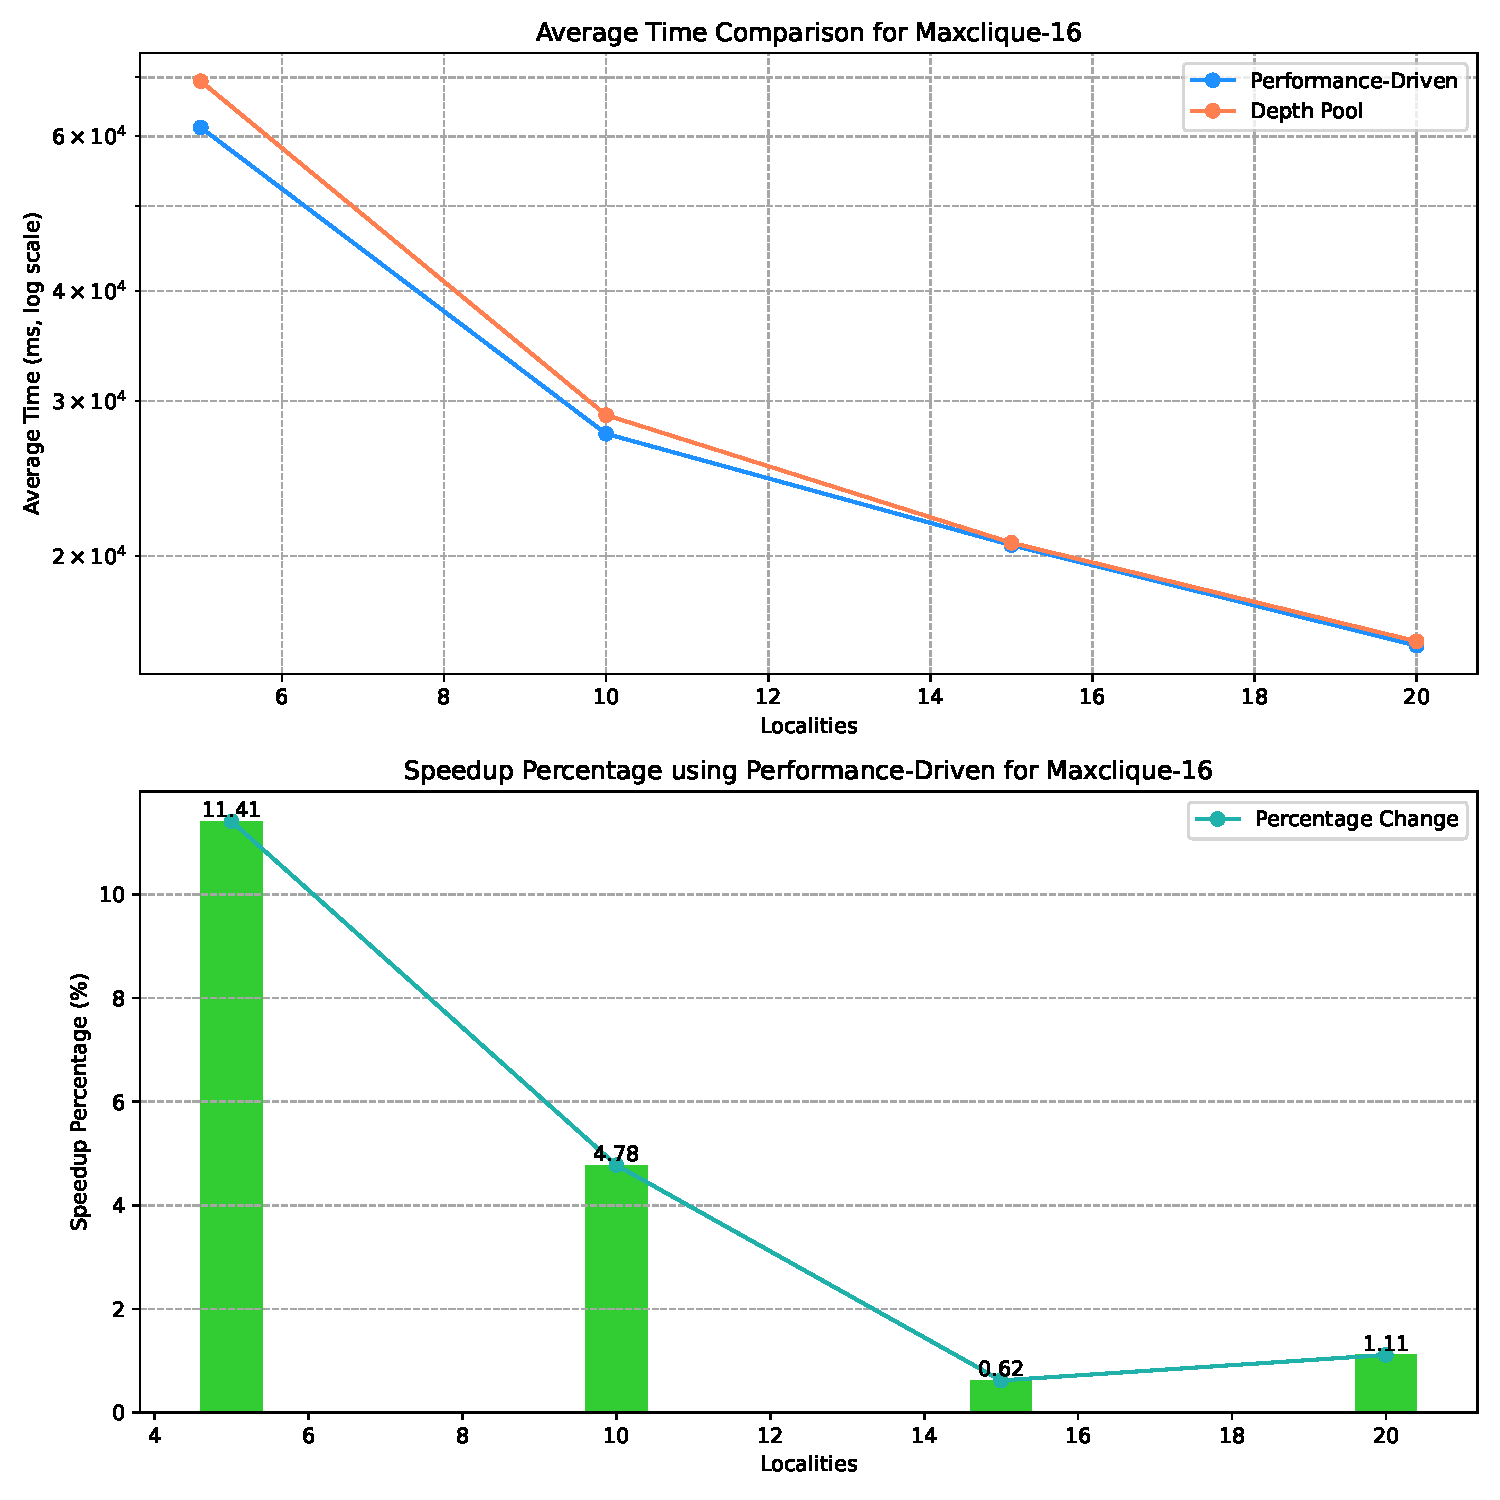
\includegraphics[width=0.98\textwidth]{images/time_comparison_max_solo.pdf} % 插入图片,设置图片宽度为文本宽度的80%
    \caption{isolated time comparison for Maxclique-16} % 提供图片的注解
    \label{fig:time_comparison_max_solo} % 为图片提供一个标签,以便在文档的其他地方引用
\end{figure}
\FloatBarrier

从图中可以看出在单独运行下,对于不同的节点数量,
基于Performance-Driven Workstealing Policy的YewPar都能比原版的DepthPool Workstealing Policy的YewPar有更好的性能,
能以更短的时间完成所有任务.

但是从图中也可以看出,在节点数量从5个到15个的区间中,
速度的提升从最高的5个节点时的11.41\%降低至最低的15个节点时的0.62\%,
之后到20节点数量时又有所提升,到了1.11\%.
而理论上节点数量越多,能够优化窃取目标的空间越大,
所以速度的提升应该是越来越明显的,
所以我们对这一现象进行了分析.
\begin{itemize}
    \item 对于Performance-Driven Workstealing Policy分析后发现,
          次要原因包含了由于节点的增加导致了系统总体由于数据收集和计算的开销增加等,
          但是理论上开销的增加相比对于优化窃取目标带来的提升是微不足道的.
    \item 从应用实现进行研究和测试的具体数据上分析后,
          发现应该主要是由于性能异常\ref{sec:performance_anomalies}的原因,
          基于Depth-Bounded skeleton的Maxclique程序相比其它应用具有更高的超线性减速的概率,
          为了验证这一推测,除了对YewPar代码进行分析外,
          我们还对基于Depth-Bounded skeleton的Maxclique程序进行了运行时间的波动情况的分析,
          以节点数量为10时的数据为例,
          其运行时间的波动情况如\cref{fig:maxclique_16_fluctuations}所示,
          \begin{figure}[h]
              \centering
              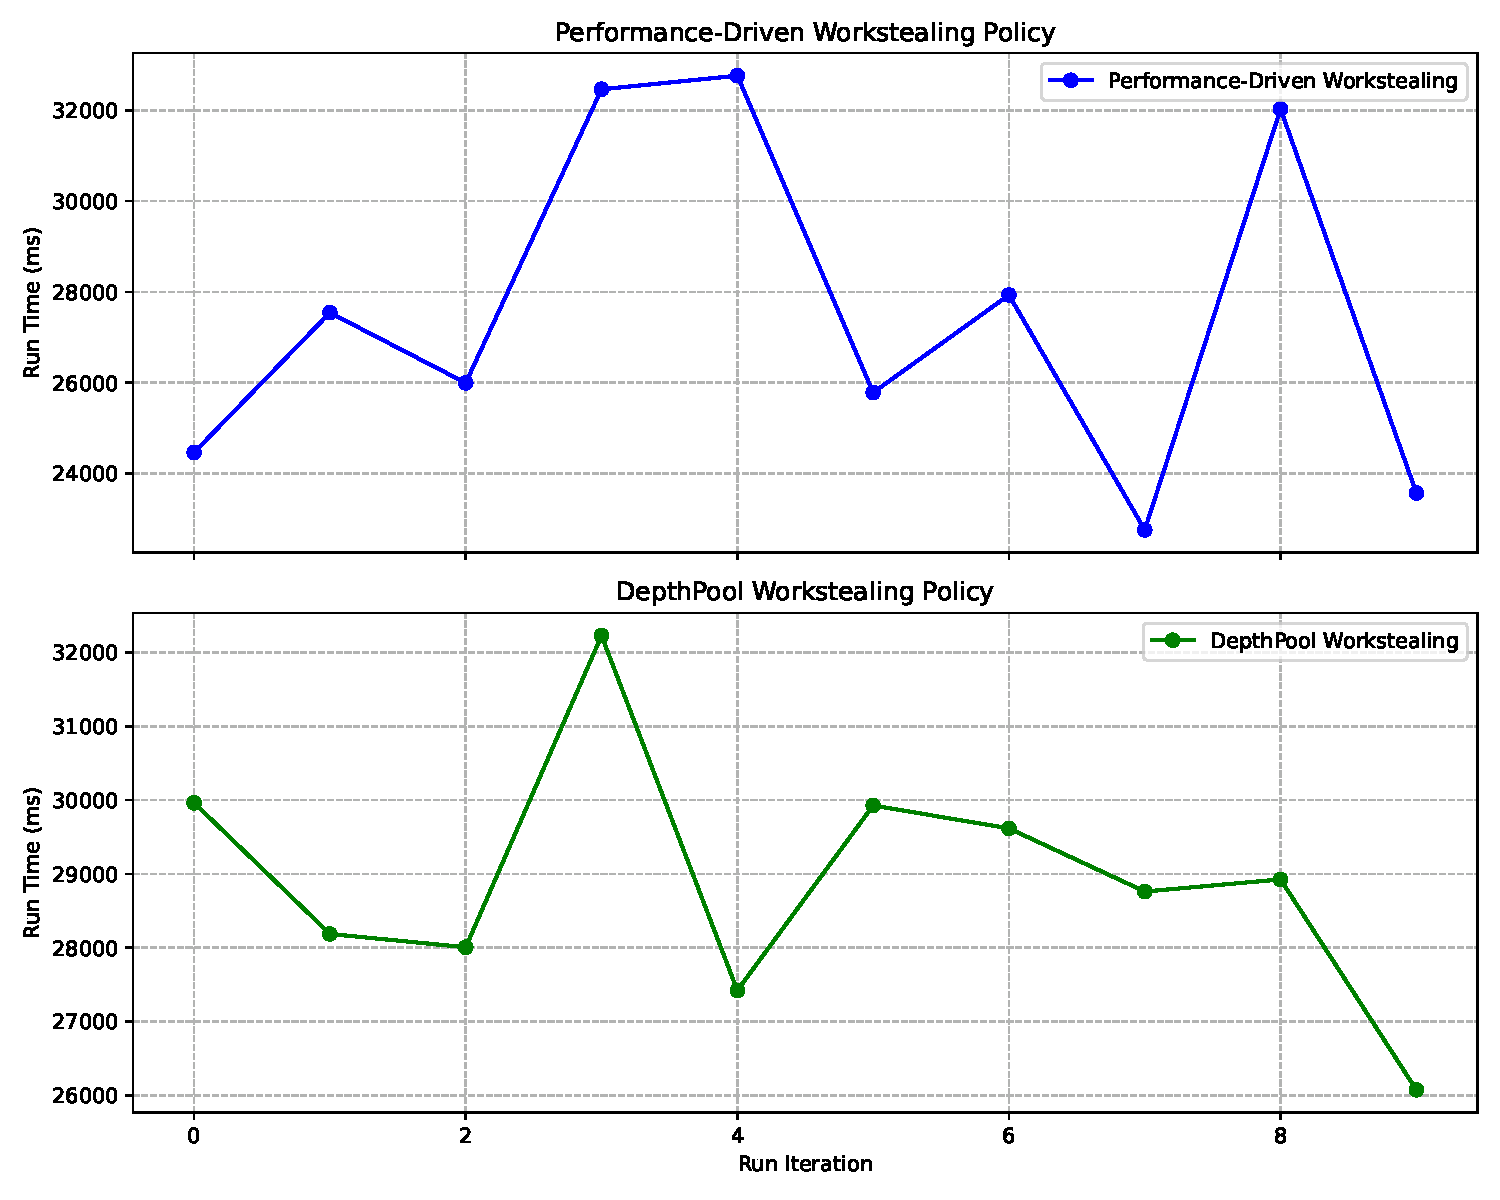
\includegraphics[width=0.8\textwidth]{images/maxclique_16_fluctuations.pdf}
              \caption{Runtime fluctuations for maxclique-16 application based on two different policies using 10 localities.}
              \label{fig:maxclique_16_fluctuations}
          \end{figure}
          在评估Maxclique-16应用的运行时间波动性时,
          我们计算了最大值与最小值之间的差异百分比.
          这可以通过以下公式得出:
          \begin{equation}
              \text{Variability Percentage} = \left( \frac{\text{Max Value} - \text{Min Value}}{\text{Min Value}} \right) \times 100\%
              \label{eq:variability_percentage}
          \end{equation}
          对于基于Performance-Driven Workstealing Policy的maxclique-16应用,
          最大差异百分比为43.98\%。
          而对于基于DepthPool Workstealing Policy的应用,
          最大差异百分比为23.61\%。
          不难看出,基于Depth-Bounded skeleton的Maxclique程序的运行时间已经具有很高的波动性,
          而基于Performance-Driven Workstealing Policy的Maxclique程序的运行时间波动性相比前者更高,几乎是其波动性的两倍.
          再结合性能异常\ref{sec:performance_anomalies}的内容,
          不难发现这里Maxclique程序对于额外的计算资源可能会更多的破坏搜索启发式方法,
          造成系统总体增加了更多的额外任务量.

          而基于Performance-Driven Workstealing Policy的maxclique-16应用由于对于窃取目标的变化更为频繁,
          由于YewPar窃取目标时的设计是从任务池右侧进行窃取,
          频繁的变换要窃取的任务池导致窃取的任务不连续,
          从而更多的导致在没有完整的左侧信息的情况下推测性地搜索子树,
          生成了更多的额外任务拖慢了程序的运行速度.
          而且更多节点时越容易导致窃取目标的变动,所以带来的速度提升会相对降低.

          由于这些数据和性能异常中描述的情况相符,从而验证了我们的推测.

          而虽然窃取目标的变动会导致额外的任务生成,
          但是我们注意到\cref{fig:time_comparison_max_solo}在15节点到20个节点数量的区间中,
          运行速度还是相对有了提升,
          应该是由于优化窃取目标带来的收益相比于额外任务带来的损耗逐渐变大导致的.
\end{itemize}


\subsection{Isolated Performance Evaluation of NS-hivert}

对于基于Budget skeleton的NS-hivert程序的每组运行时间测试各进行十次取平均值后的结果如\cref{fig:time_comparison_ns_solo}所示,
也分为运行时间评估与基于Performance-Driven Workstealing Policy比原来的DepthPool Workstealing Policy的运行速度提升评估两个部分.

\begin{figure}[h]
    \centering % 让图片居中显示
    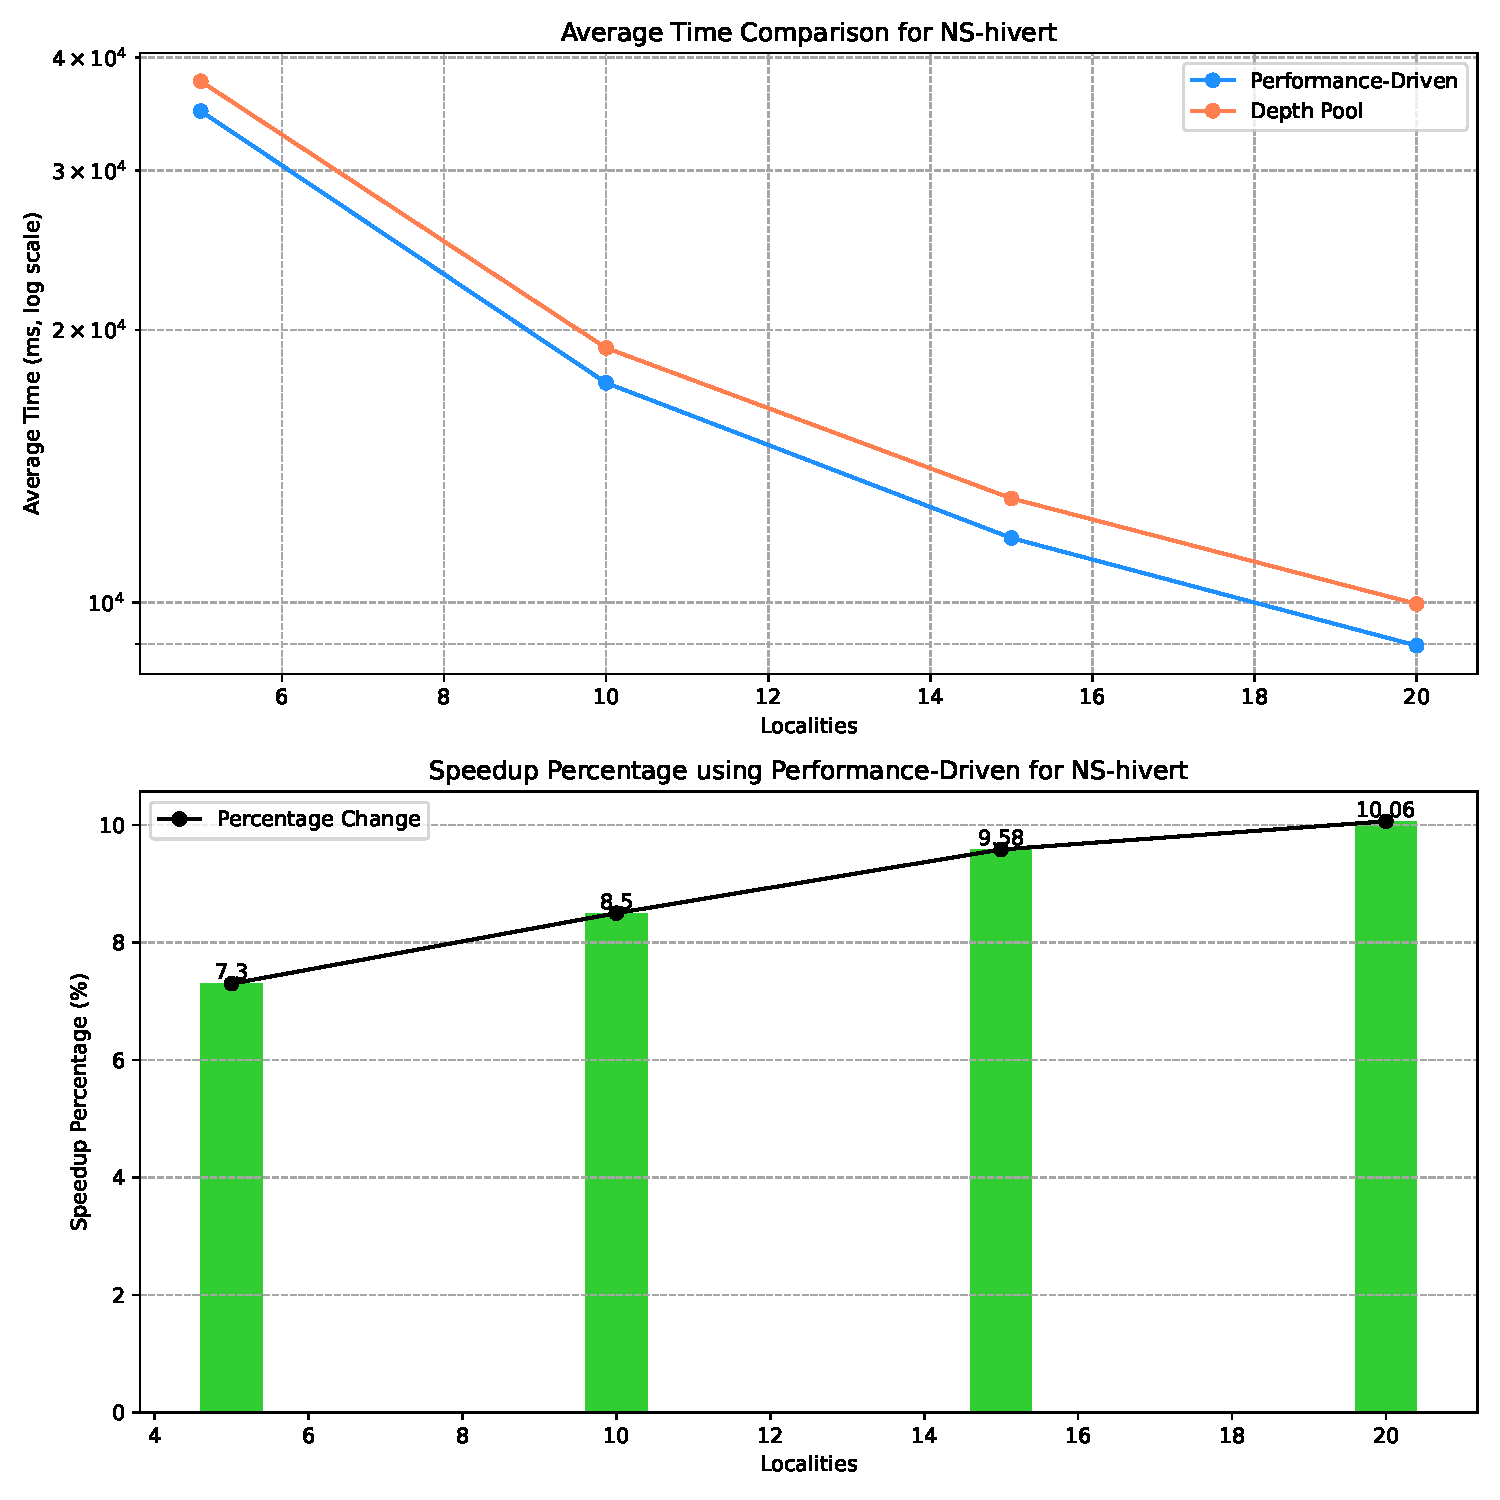
\includegraphics[width=0.98\textwidth]{images/time_comparison_ns_solo.pdf} % 插入图片,设置图片宽度为文本宽度的80%
    \caption{isolated time comparison for NS-hivert} % 提供图片的注解
    \label{fig:time_comparison_ns_solo} % 为图片提供一个标签,以便在文档的其他地方引用
\end{figure}
\FloatBarrier

可以看出在单独运行的情况下,
基于Performance-Driven Workstealing Policy的NS-hivert程序在不同节点数量都具有更优的性能,
能以更短的时间完成所有任务.
其中速度的提升随着节点数量的增加而增加,
在节点数量为20时,速度的提升达到了平均10.06\%,
考虑到这只是通过调整Workstealing Policy达到的整体速度提升,
并没有对YewPar其它部分进行改动,
并且有性能异常\ref{sec:performance_anomalies}等其它因素产生的负面影响,
所以这一结果已经是非常优秀的.

相比于Maxclique程序,
这里节点数量增多时使用Performance-Driven Workstealing Policy带来的速度提升更为明显,
这是由于NS-hivert程序运行时性能异常\ref{sec:performance_anomalies}产生的负面影响较小,
同样我们对NS-hivert程序的运行时间波动性进行了分析,
如\cref{fig:NS_hivert_fluctuations}所示.

\begin{figure}[h]
    \centering
    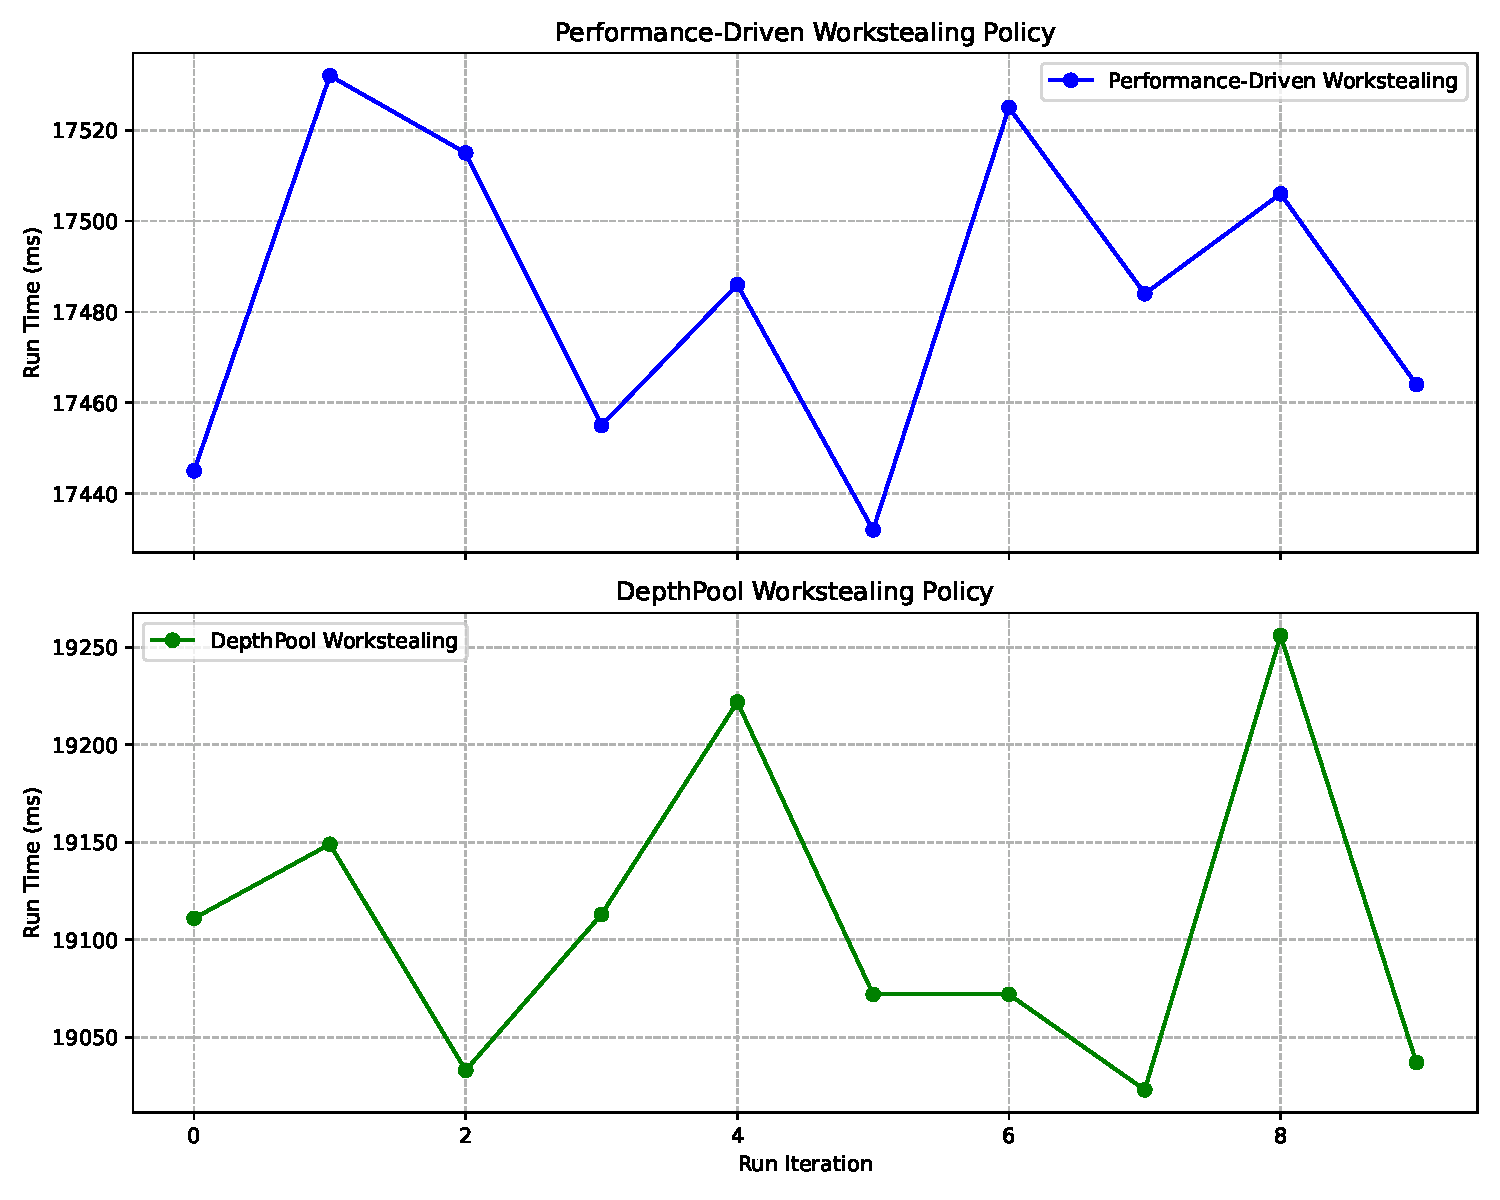
\includegraphics[width=0.8\textwidth]{images/NS_hivert_fluctuations.pdf}
    \caption{Runtime fluctuations for Maxclique-16 application based on two different policies using 10 localities.}
    \label{fig:NS_hivert_fluctuations}
\end{figure}
\FloatBarrier

通过使用\cref{eq:variability_percentage}进行最大差异百分比计算,
对于基于Performance-Driven Workstealing Policy的maxclique-16应用,
最大差异百分比为0.57\%。
而对于基于DepthPool Workstealing Policy的应用,
最大差异百分比为1.22\%。
这相对于Maxclique程序的运行时间波动性是非常小的,
所以推测出NS-hivert程序运行时变更任务执行顺序产生的超线性减速概率较小.
这时速度提升的主要原因应该是由于优化窃取目标带来的收益导致的.


\section{Simultaneous Performance Evaluation under Resource Contention}

这里主要评估在各节点的计算资源不均衡,有争用的情况下,
基于新的Performance-Driven Workstealing Policy的YewPar与原版在性能上的差异.
因为实际部署环境可能很复杂,
不同节点有不同的计算资源占用情况,
通过对比在资源争用的情况下Performance-Driven Workstealing Policy的表现,
能够更全面地评估其性能.

为了模拟不同节点的计算资源占用情况,
我们使用了一种简单的方法,
通过直接同时运行基于不同Policy的YewPar程序,
让两种程序在同一时间内同时运行,
由于两种程序设置的各节点使用的线程数均和各节点的所拥有的核心数相同,
从而产生较为严重的资源争用,
而由于原版的DepthPool Workstealing Policy所采用的策略是偏随机窃取的,
所以也能够较好地模拟负载不均衡的情况下的资源争用.

但是这样会产生一个问题,
就是当其中一个程序运行完毕后,
剩下的程序会重新独占所有的计算资源,
所以下面评估结果中Performance-Driven Workstealing Policy所产生的性能提升会相对实际情况有所低估,
但是这样的评估结果仍然能够反映出两种Policy在各节点的计算资源不均衡和争用的情况下的性能差异.

\subsection{Simultaneous Performance Evaluation of Maxclique}

对于基于Depth-Bounded skeleton的Maxclique程序的每组同时运行情况下的运行时间测试,各进行十次取平均值后的结果如\cref{fig:time_comparison_max_simu}所示,
其中也分为运行时间评估与基于Performance-Driven Workstealing Policy比原来的DepthPool Workstealing Policy的运行速度提升评估两个部分.

\begin{figure}[h]
    \centering % 让图片居中显示
    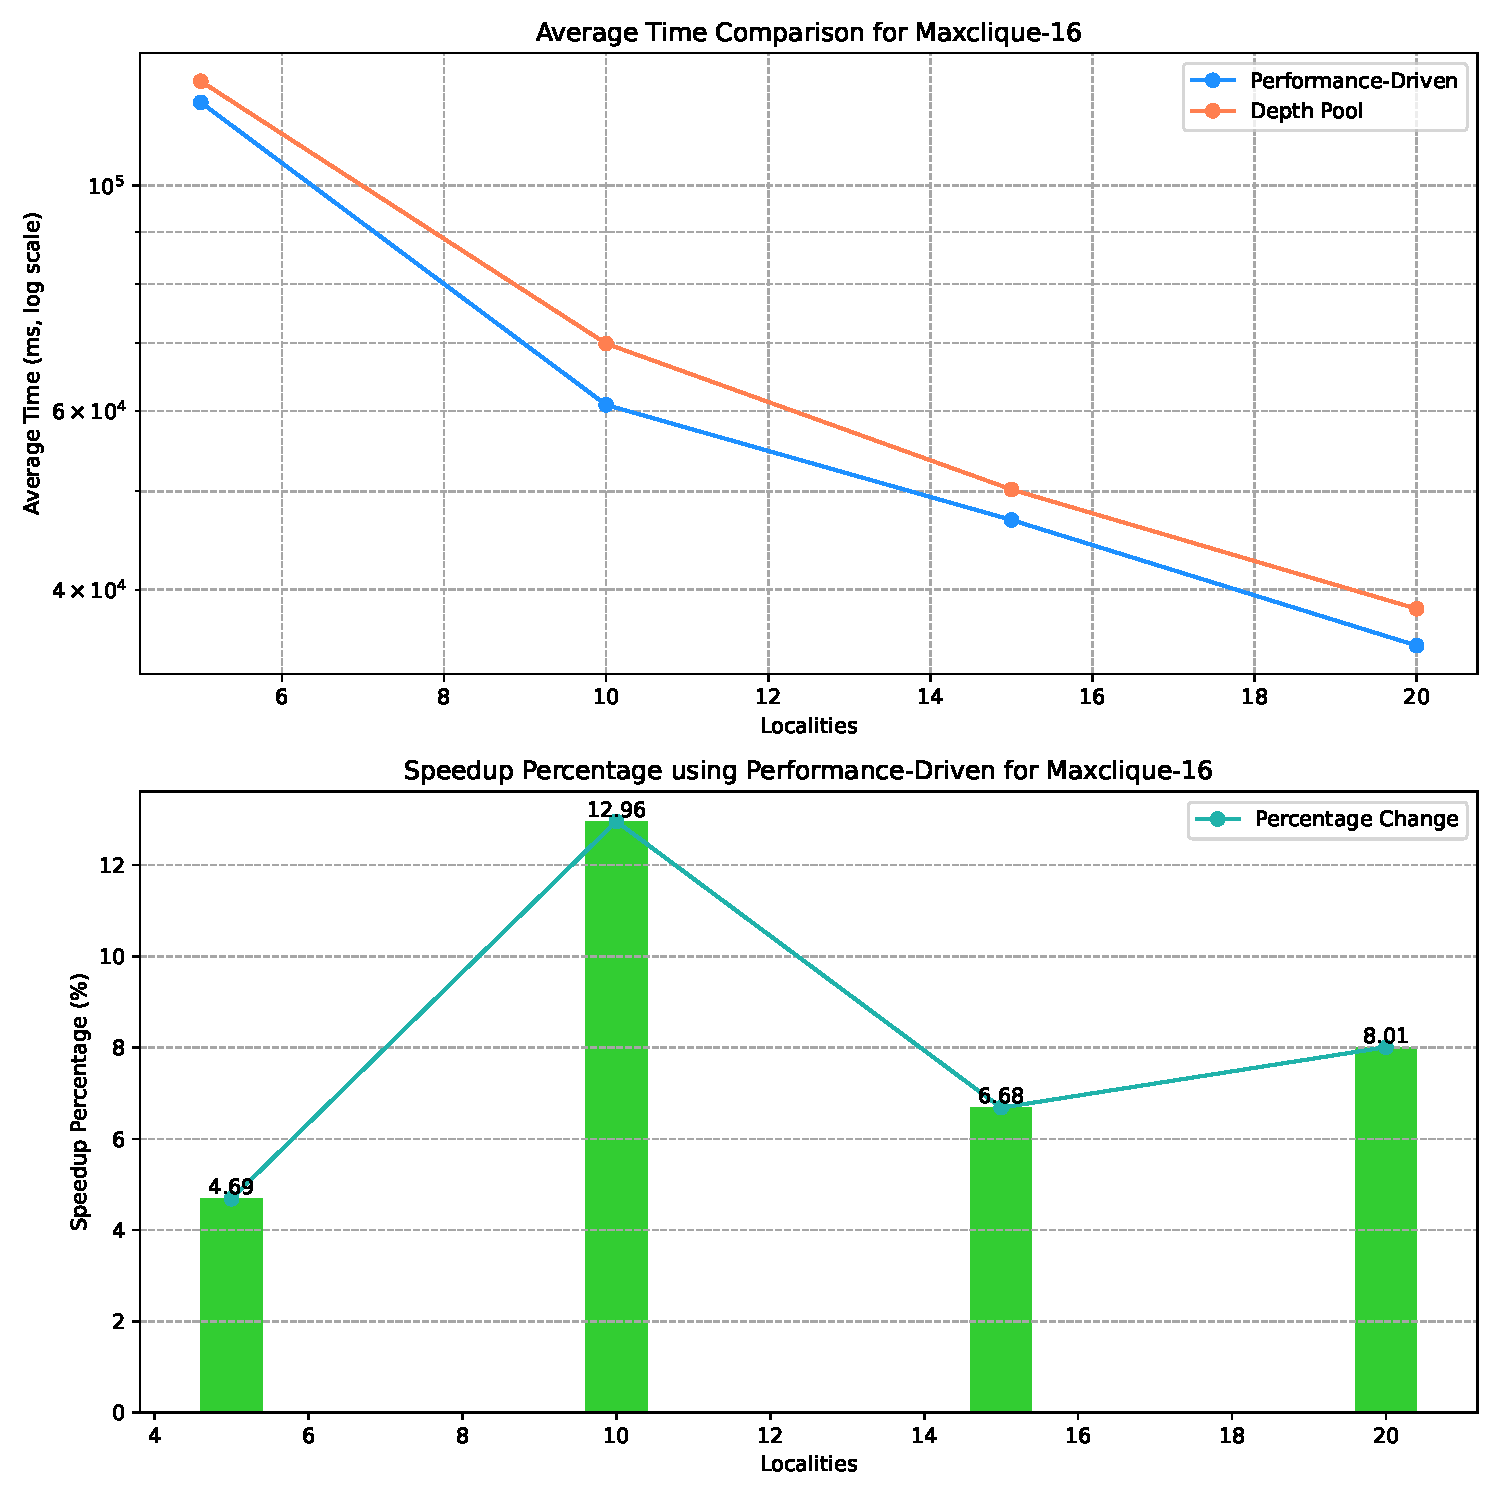
\includegraphics[width=0.98\textwidth]{images/time_comparison_max_simultaneously.pdf} % 插入图片,设置图片宽度为文本宽度的80%
    \caption{simultaneous time comparison for Maxclique-16} % 提供图片的注解
    \label{fig:time_comparison_max_simu} % 为图片提供一个标签,以便在文档的其他地方引用
\end{figure}
\FloatBarrier

可以看出Maxclique虽然有较为严重的超线性减速的情况,
但是在各节点负载不均衡的情况下,
基于Performance-Driven Workstealing Policy的Maxclique应用的运行速度优势有了明显的提升.
例如在节点数量为20时,速度提升比例从单独运行时的1.11\%提升至了同时运行时的8.01\%,
提升了接近8倍.
推测这是由于在负载不均衡的情况下,
优化窃取目标带来的优势明显大过了额外任务带来的损耗.
同时从图中可以看出,
在节点数从10到15时,
额外任务的损耗降低了一些运行速度的提升,
但是随着节点数的增多,
优化窃取目标带来的优势又开始逐渐显现.


\subsection{Simultaneous Performance Evaluation of NS-hivert}

对于基于Budget skeleton的NS-hivert程序的每组同时运行情况下的运行时间测试,各进行十次取平均值后的结果如\cref{fig:time_comparison_ns_simu}所示,
其中也分为运行时间评估与基于Performance-Driven Workstealing Policy比原来的DepthPool Workstealing Policy的运行速度提升评估两个部分.

\begin{figure}[h]
    \centering % 让图片居中显示
    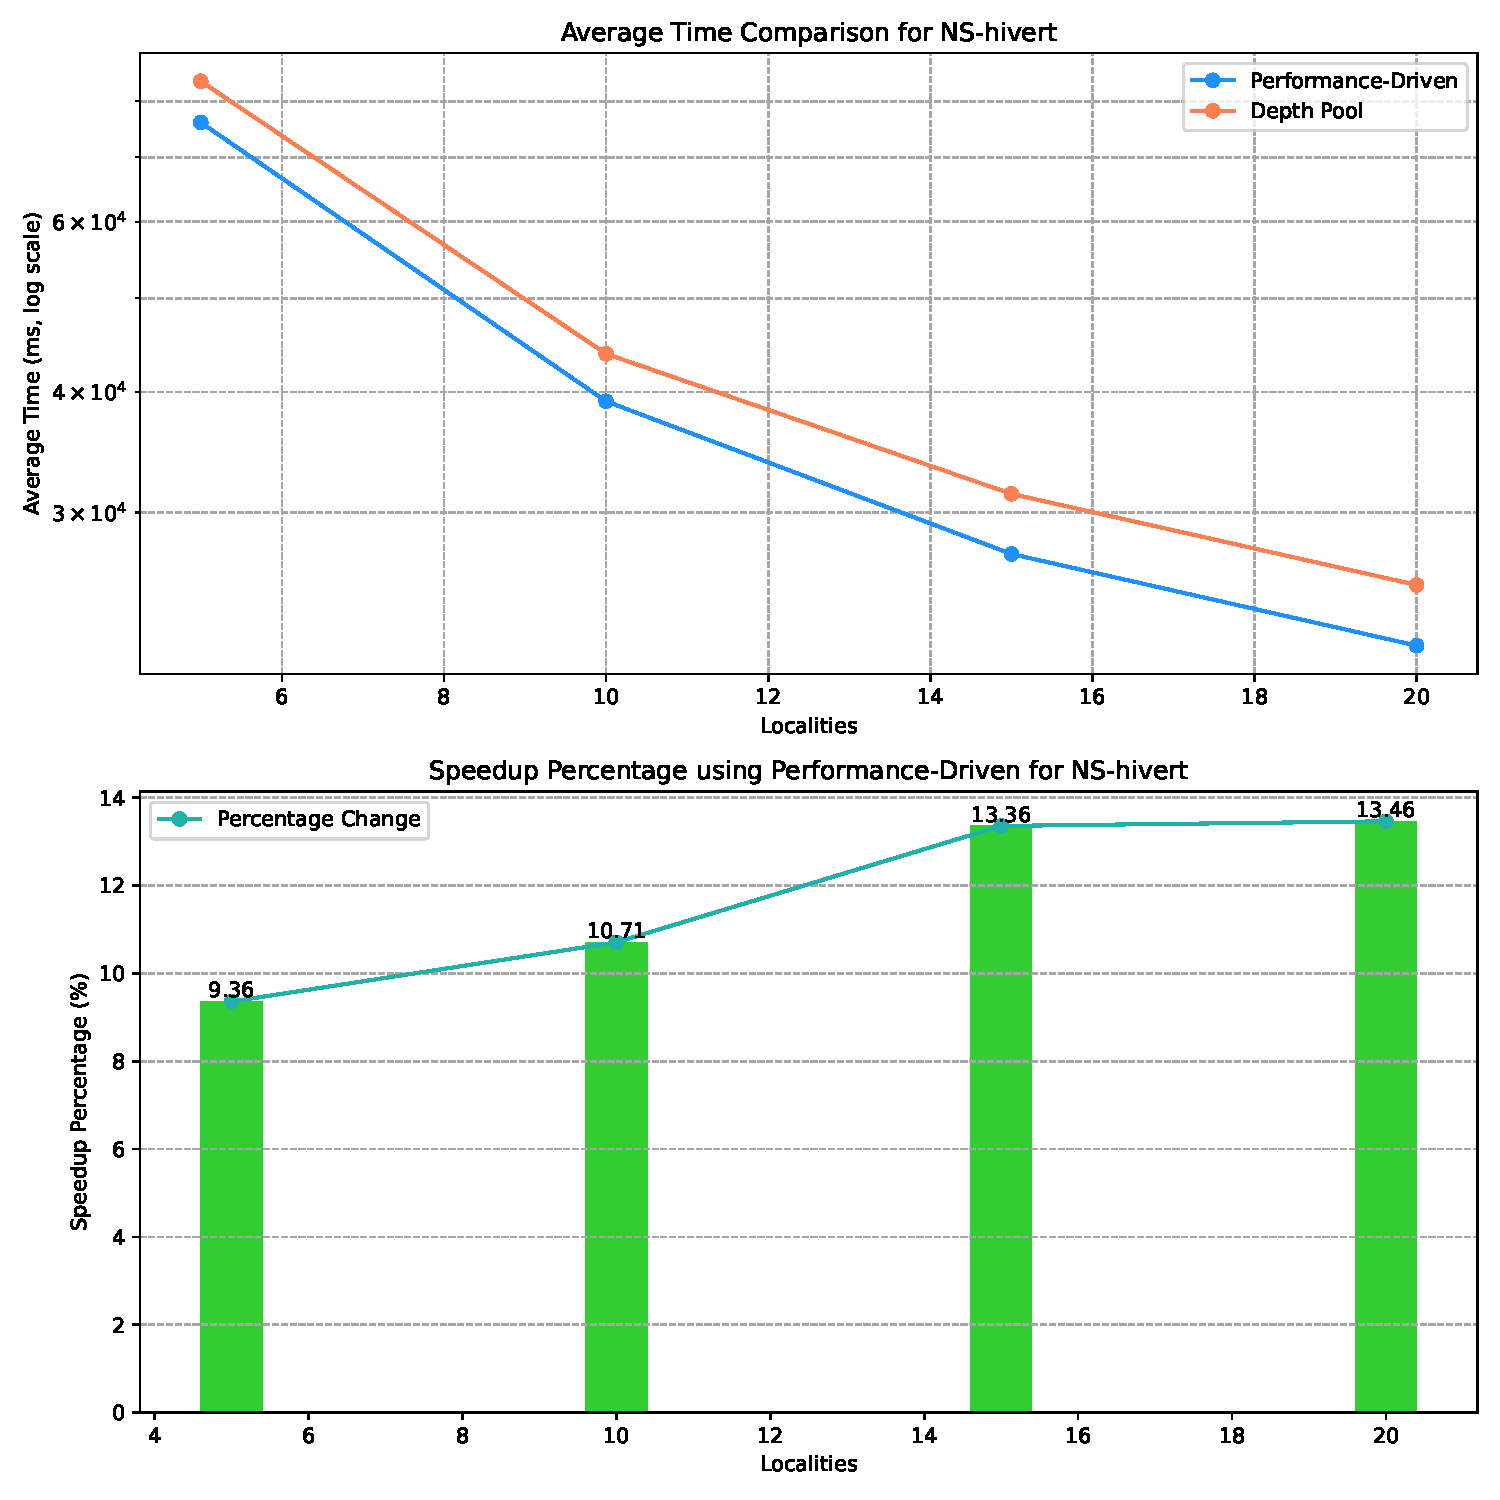
\includegraphics[width=0.98\textwidth]{images/time_comparison_ns_simultaneously.pdf} % 插入图片,设置图片宽度为文本宽度的80%
    \caption{simultaneous time comparison for NS-hivert} % 提供图片的注解
    \label{fig:time_comparison_ns_simu} % 为图片提供一个标签,以便在文档的其他地方引用
\end{figure}
\FloatBarrier

从图中可以看出在基于Budget skeleton的NS-hivert程序中,
Performance-Driven Workstealing Policy对于性能的提升更加明显,
从5个节点数时的9.36\%逐步提升至20个节点时的13.46\%,
考虑到Workstealing Policy相对于整个YewPar框架和NS-hivert程序的优化空间很小,
所以达到13.46\%的性能提升是非常优秀的.

从图中节点数从15到20时的很小的提升幅度可以推测,
随着节点数增加带来的性能提升比例已经接近于Workstealing部分可提升的极限,
其它程序运行的时间大多消耗在处理任务和YewPar框架的其它开销上.

\section{Performance-driven Workstealing Policy framework additional Performance cost Evaluation}

为了探究Performance-Driven Workstealing Policy的轻量化设计是否对性能有明显的额外损耗,
我们在仅使用一个节点下的一个worker(仅占用一个线程)的情况下对比不同Policy下的NS-hivert应用的运行时间.
使用NS-hivert应用因为它的运行时间波动较小,造成的干扰较小,
为了缩短运行时间方便测量,
我们将其参数g改为$g = 37$(genus: Depth in the tree to count until).

测试结果如\cref{fig:time_comparison_ns_one_worker},
\begin{figure}[h]
    \centering % 让图片居中显示
    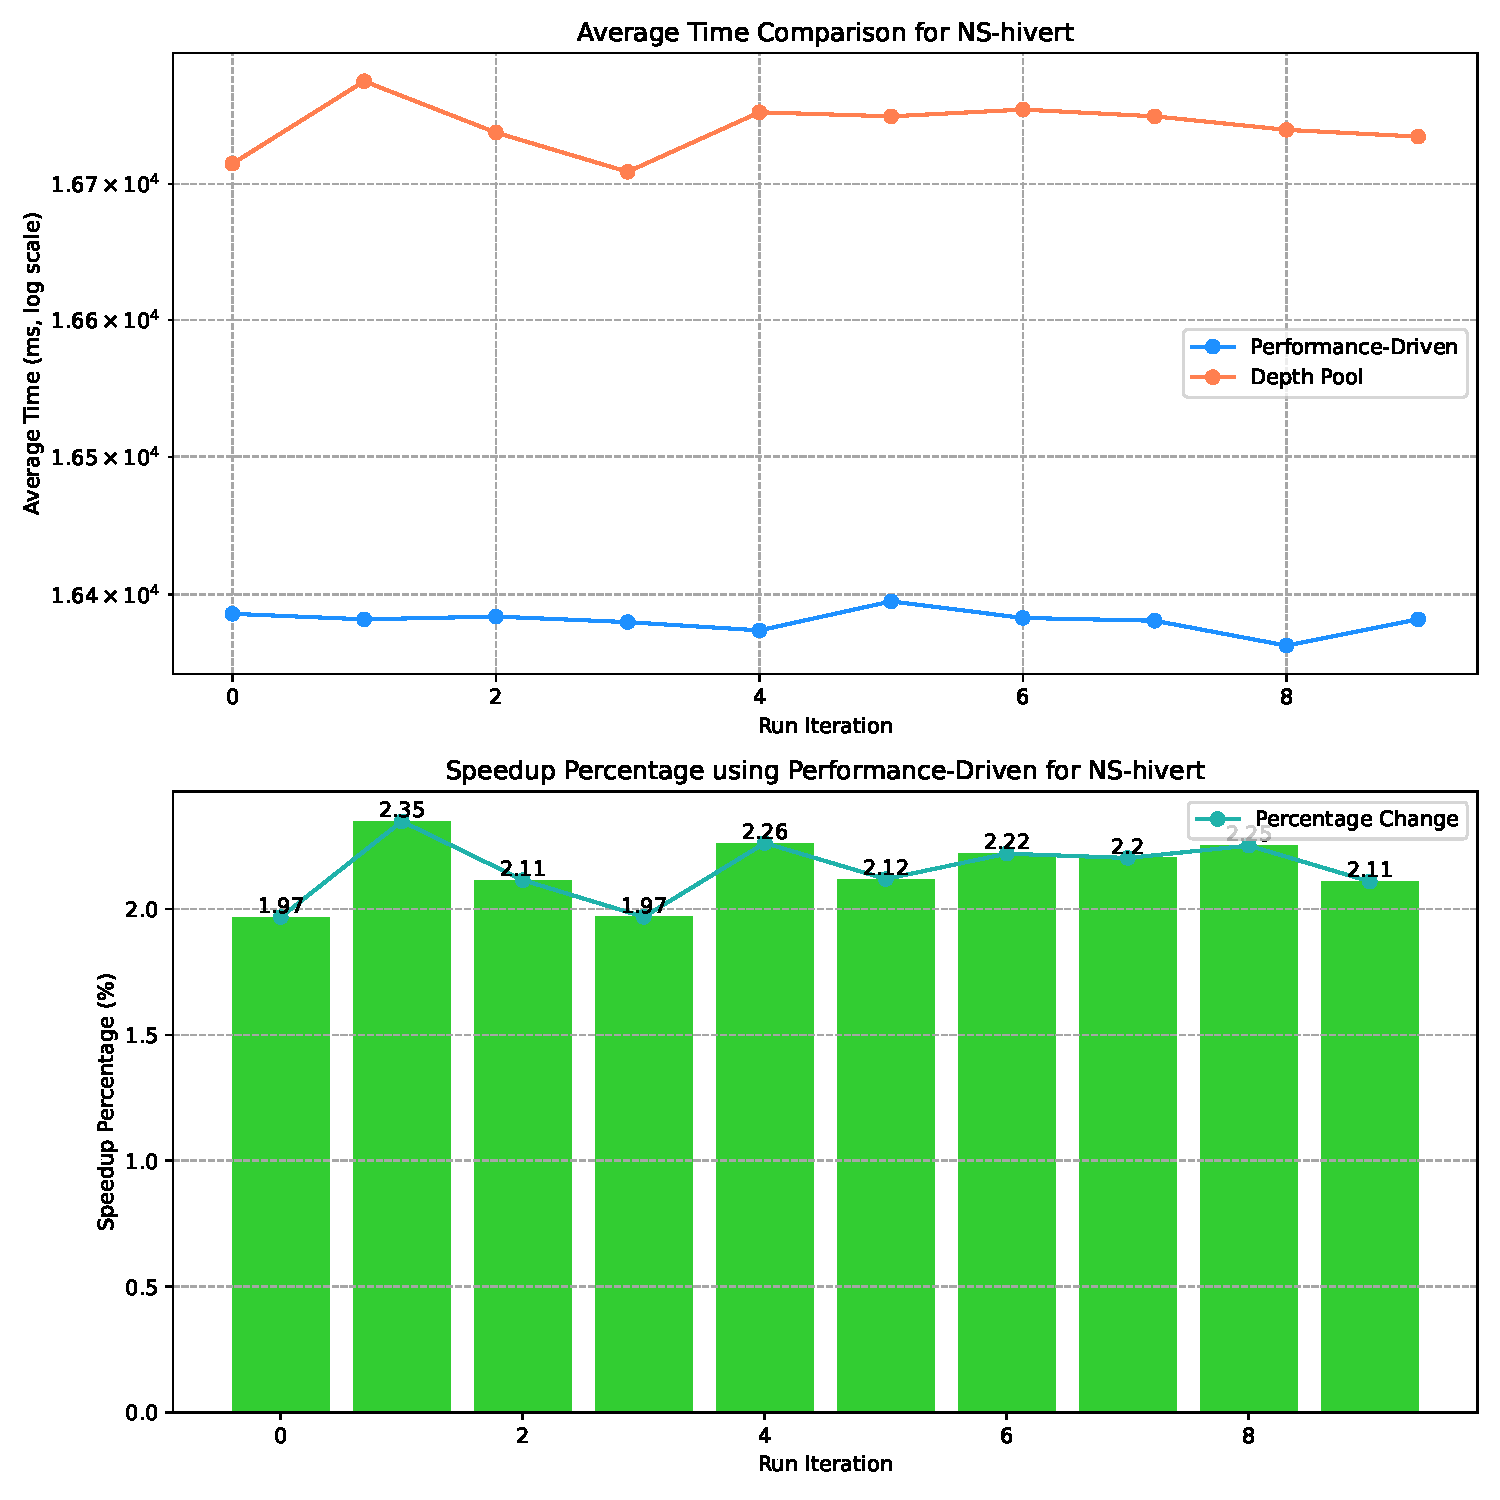
\includegraphics[width=0.98\textwidth]{images/time_comparison_ns_one_worker.pdf} % 插入图片,设置图片宽度为文本宽度的80%
    \caption{time comparison for NS-hivert using one locality with one worker} % 提供图片的注解
    \label{fig:time_comparison_ns_one_worker} % 为图片提供一个标签,以便在文档的其他地方引用
\end{figure}
\FloatBarrier

可以看出由于Performance-Driven Workstealing Policy的轻量化设计,
通过无锁化等机制减少了计算资源的额外损耗,
在仅使用单个worker,
无任务窃取发生的情况,也就是无法优化窃取目标的情况下,
而且在Performance-Driven Workstealing Policy有后台任务动态刷新窃取目标的情况下,
也能比原版YewPar的Workstealing Policy的应用达到2\%左右的速度提升,
说明其设计是非常成功的,
成功达到了轻量化的目的,
减少了因为任务窃取框架带来的性能损耗.

%%%%%%%%%%%%%%%%%%%%%%%%%%%%%%%%%%%%%%%%%%%%%%%%%%%%%%%%%%%%%%%%%%%
\chapter{Conclusion}\label{conclusion}

我们的目标是通过改进YewPar的Workstealing策略来提高其性能,
为此设计并实现了一种通过各节点的各项性能数据来优化Workstealing时的窃取目标的Performance-Driven Workstealing Policy,
其中包含性能数据的收集,处理,传输,
,对于最优窃取目标的计算和缓存,
以及一套包含两种方式的刷新机制.
通过针对多线程和多节点通讯的优化设计,
以很低的成本实现了对于程序运行速度的提升,
并具有很好的兼容性.

从评估结果来看,
我们的Performance-Driven Workstealing Policy在Workstealing方面的优化效果是非常明显的,
在无计算资源占用的情况下,
运行程序速度的提升已经能达到8\%以上,
而在各节点资源占用不均衡,有争用的情况下,
运行程序速度的提升能高达到13\%以上.
考虑到这只是通过优化YewPar中的Workstealing Policy达到的整体速度提升,
而程序大部分时间花在处理任务和生成新的任务等情况上,
所以通过各节点程序的性能数据调整窃取目标的方法是非常有效的,
而Performance-Driven Workstealing Policy在不同情况都是非常优秀的Workstealing Policy,
完全可以取代YewPar原先的Workstealing Policy.

\section{future work}

\subsection{各项参数的自动调整}

在之前的\ref{design}章节中,
程序有一些算法的固定参数例如指数平滑算法中的历史数据所占比例是根据测试得出的一个较优的值,
而在实际更复杂的情况下,
这些参数可能有更优的选择和具有更多优化的空间,
所以可以考虑通过设计一套自动调整这些参数的算法,
来保障各种情况下Performance-Driven Workstealing Policy内部的各种参数都能达到一个较优的状态.

\subsection{针对并行组合搜索的性能异常情况的优化}

在之前的评估环节可以看出Maxclique程序下,
Performance-Driven Workstealing Policy对于窃取目标的频繁变动更多地破坏了搜索启发式方法,
打乱了任务执行的顺序,
导致了更多的额外用于推测上下文的任务生成,
从而拖慢了程序的整体运行速度,
可以考虑设计一套算法将避免破坏任务执行的顺序也包含在计算窃取目标的过程中,
可能能减少额外任务的生成,
从而进一步提升程序在多节点多线程情况下的运行速度.

\subsection{替代全部的YewPar Workstealing Policy}

Performance-Driven Workstealing Policy目前替代了例如YewPar中的DepthPool Policy,
从而提升了YewPar中的一些skeleton的性能,
但是由于时间原因还未去尝试替代例如Priority Ordered Policy,
所以暂时未能让YewPar的全部skeleton都能受益于Performance-Driven Workstealing Policy.
这个可以作为后续的工作进行尝试.


\appendix % first appendix
%%%%%%%%%%%%%%%%%%%%%%%%%%%%%%%%%%%%%%%%%%%%%%%%%%%%%%%%%%%%%%%%%%%
\chapter{First appendix}

\section{Section of first appendix}

%%%%%%%%%%%%%%%%%%%%%%%%%%%%%%%%%%%%%%%%%%%%%%%%%%%%%%%%%%%%%%%%%%%
\chapter{Second appendix}

%%%%%%%%%%%%%%%%%%%%%%%%%%%%%%%%%%%%%%%%%%%%%%%%%%%%%%%%%%%%%%%%%%%
% it is fine to change the bibliography style if you want
\bibliographystyle{plain}
\bibliography{mproj}
\end{document}
